\newgeometry{textwidth=16cm}
\chapter[Discerning inter- and intramolecular vibrations]{Discerning inter- and intramolecular vibrations of sulfur polyaromatic compounds}
\minitoc
\restoregeometry

\newpage	
	
\vspace*{6cm}	
	\textit{Thiophenes are an important class of molecules in fields as diverse as petrochemistry, molecular electronics, and optoelectronics. Thiophenic submolecular motifs are thought to play a role in molecular association and nano-aggregation phenomena in both pure materials and natural and synthetic mixtures. Vibrational (infrared and Raman) spectroscopy provides the means to characterize these species. In this work far-infrared photoacoustic and low-frequency Raman spectra of a series of polycyclic aromatic hydrocarbons containing sulfur have been measured and interpreted using DFT calculations based on a perturbational-variational method coupled with potential truncation. The approach and outcomes illustrate how inter- and intramolecular vibrations for thiophenic systems in single and multicomponent mixtures can be discriminated. This work offers the perspective to search the inter- and intra-molecular signatures of the main submolecular motifs and heteroelements postulated as being present in the asphaltenes.}


	\newpage
	
	\section{Introduction}
	
	Thiophenes are an important class of molecules in various domains of chemistry including petrochemistry, \cite{waldo1991sulfur,mitra1998determination,lobodin2015separation}  molecular electronics,\cite{katz2004recent,ong2008thiophene,vivas2011linear,silva2011controlling} and optoelectronics.\cite{kim2010one} In particular, they are of great interest in all that concerns oil upgrading. \cite{kishita2003upgrading,samokhvalov2011heterogeneous,chen2015acylation} Their presence as aromatic fragments in asphaltenes has been revealed by methods such as thermolysis analysis,\cite{strausz1992molecular} mass spectroscopy,\cite{liu2010molecular,karimi2011quantitative}  and NMR and IR spectroscopies. \cite{coelho2012elucidation,alhumaidan2016impact} Importantly, thiophenes are hypothesized to play a key role in the aggregation of asphaltenes\cite{widany2001electronic,liu2014adjusting} which is of uppermost importance to the oil extraction process. Asphaltenes are known to cause the blocking of pipelines and refinery equipment.\\
	
	The molecular structure of asphaltenes is difficult to determine since they are formed by thousands of molecules that tend to stick together in solution. Over the past six decades, the composition, molecular structure and colloidal state of asphaltenes in crude oil and bitumen have been considered a central enigma of petroleum chemistry.\cite{speight2014chemistry} The noncovalent interactions responsible for molecular recognition among components determine the microstructure of the aggregates. Two contrasting molecular architectures have been proposed to describe the dominant molecular motifs in asphaltenes: the island model in which asphaltene molecules contain one polyaromatic core with pendant aliphatic chains; and the archipelago model in which several aromatic motifs are bridged together via aliphatic chains.\cite{mullins2012advances,sheremata2004quantitative} Interactions indicated by the island model are dominated by $\pi$-stacking among polyaromatic cores and steric repulsion among pendant chains. In the archipelago model diverse interactions arise from van der Waals forces, hydrogen bonding and interactions among heteroatom groups. Porphyrins also play major roles. The identification of interactions in asphaltenes, the understanding of how they influence molecular arrangements, and finally the experimental method by which they are identified, are major issues in production, transport, and refinery system design and operation.\cite{speight1999desulfurization} For example, understanding the impact of inter- and intramolecular interactions occurring between thiophene-like molecules is a missing and necessary refinement to asphaltene aggregation models,\cite{groenzin1999asphaltene,mackie2010importance,mullins2012advances} that will lead to better process designs for cracking asphaltene aggregates and facilitate refining of thiophene-rich crude oils.\\
	
	Several types of interactions coexist among aromatic molecules containing sulfur, mainly $\pi$-$\pi$-stacking between aromatic rings, and $\pi$-S between an aromatic ring and a sulfur atom. The interaction between aromatic rings and sulfur atoms has been shown by Morgan \textit{et al}\cite{morgan1978chains}  to play an important role in stabilizing the folded conformations of 8 different proteins. Tauer \textit{et al}\cite{tauer2005estimates} studied the H$_{2}$S-benzene dimer system in order to visualize molecular structures resulting from sulfur-$\pi$ interactions, and to establish an appropriate computational method capable of describing these interactions. The interactions driving the spatial arrangement of thiophene molecules have been studied theoretically by Tsuzuki \textit{et al}\cite{tsuzuki2002model} who showed that the major interaction among thiophene molecules was dispersive, whereas the electrostatic interactions were responsible for the orientation of the molecules.\\
	
	In our previous work,\cite{spillebout2014discerning} we showed that interactions responsible for $\pi$-$\pi$ stacking for acene molecules could be visualized in infrared and Raman spectra. The frequencies related to these interactions were found between 15 and 100 cm$^{-1}$. This range of frequencies is difficult to measure experimentally using conventional methods but with the development of terahertz spectroscopy, including synchrotron-based photacoustic (PA) IR measurements, it is now possible to identify absorption bands specific to intermolecular interactions that occur at very low frequencies and to evaluate their importance.\\
	
	In the current study we (1) identify the presence of thiophene-type molecules in complex systems, (2) identify $\pi$-stacking interactions when they are predominant in a complex system by means of vibrational spectroscopy experiments and high-precision quantum mechanical calculations, and (3) develop a new variation-perturbation method adapted to the resolution of the vibrational Schrödinger equation at very low wavenumbers for large-size systems (bigger than 15 atoms) and their dimers. These results are used to characterize and identify IR and Raman signatures of vibration modes found at very low wavenumbers that are characteristic of association, e.g. dimerization. More specifically, infrared and Raman spectra of benzothiophene \textbf{1\textit{a}}, dibenzothiophene \textbf{1\textit{b}}, 4.6-dimethyldibenzothiophene \textbf{1\textit{c}} and 4-methyldibenzothiophene \textbf{1\textit{d}} are reported. The observed bands are assigned using high level calculations based on anharmonic electrical and mechanical approximations. Fundamental bands previously assigned by Bree \textit{et al}\cite{bree1971vibrations} are confirmed, and additional combination bands are identified. The approach and outcomes illustrate how inter- and intramolecular vibrations in single- and multi-component mixtures can be discriminated.
	
	\begin{figure}[H]
		\centering
		%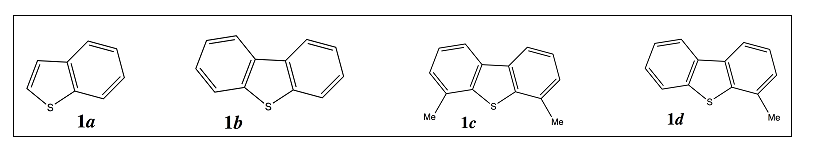
\includegraphics[scale=0.7]{image/P1-F1}
		\caption{Molecular structures studied:  from left to right: benzothiophene \textbf{1\textit{a}}, dibenzothiophene \textbf{1\textit{b}}, 4.6-dimethyldibenzothiophene \textbf{1\textit{c}} and 4-methyldibenzothiophene \textbf{1\textit{d}}}
	\end{figure}
	
	
	\section{Experimental Spectra}
	
	Dibenzothiophene \textbf{1\textit{b}}, 4.6-dimethyldibenzothiophene \textbf{1\textit{c}} and 4-methyldibenzothiophene \textbf{1\textit{d}} were obtained from commercial sources at purity levels of at least 98 per cent and analyzed as received. In some cases, samples were ground manually prior to acquisition of their spectra. 
	
	\bigskip
	
	\subsection{Raman spectra}	

	Raman spectra were obtained using two spectrometers at CanmetENERGY (Devon, Alberta). In one set of experiments, a Renishaw InVia microscope-based system was coupled to a Spectra Physics 125 He-Ne laser, which provided excitation at 633 nm. Several milligrams of each solid were examined with the use of a 50$\times$microscope objective. Spectra were acquired with a spherically focused incident beam; typical resolution was better than 2 cm$^{-1}$. Total accumulation time was 5 min for each spectrum. The second group of experiments was performed with a Bruker IFS 88 FT spectrometer and FRA 106 Raman accessory. Excitation of the FT-Raman spectra was effected with a 1064-nm Nd:YAG laser at power levels between 90 and 260 mW. Ten 32-scan spectra with a resolution of 8 cm$^{-1}$ were averaged for each sample. \\
	
	\subsection{Far-infrared spectra}
	
	\bigskip
	
	PA far-infrared spectra were acquired at a resolution of 6 cm$^{-1}$ using two different Bruker IFS 66v/S Fourier transform infrared (FT-IR) spectrometers. The first instrument, at CanmetENERGY, was operated in both rapid- and step-scan modes. The He-Ne laser modulation frequency was 1.6 kHz for the rapid-scan measurements. Large amplitude phase modulation\cite{michaelian2009far} was employed in the step-scan experiments, with a Signal Recovery lock-in amplifier being utilized for demodulation. The second spectrometer was located at the Canadian Light Source (Saskatoon, Saskatchewan). Rapid-scan spectra were acquired under conditions similar to those just mentioned. A thermal (globar) source was employed with this instrument.\\
	
	Standard MTEC 300 gas-microphone PA accessories were used with both spectrometers; the sample cells were fitted with polyethylene windows. Helium was employed as the carrier gas. Multilayer mylar beam splitters were installed in the interferometers. Spectra were recorded between about 50 and 700 cm$^{-1}$, due to limits imposed by the optical materials. Carbon black powder or an MTEC carbon black reference yielded reference spectra that were used to correct sample spectra for the wavenumber-dependent response of each instrument.\\
	
	\subsection{Mid-infrared spectra}
	
	\bigskip
	
	PA mid-infrared spectra were recorded at a resolution of 6 cm$^{-1}$ using the Bruker IFS 88 spectrometer mentioned above. The laser frequency was either 1.6 or 2.2 kHz. An MTEC 200 PA cell was utilized. Nitrogen was used to purge the spectrometer and as a carrier gas. A KBr window sealed the PA cell, and a Ge/KBr beam splitter was used in the spectrometer. Ten 32-scan spectra were averaged for each sample. Spectra were acquired from about 400 to 4000 cm$^{-1}$. Carbon black powder was used to obtain reference spectra in these experiments.
	
	
	\section{Calculation method for thiophene-type molecules and their dimers}
	
	\subsection{Structural details }
	
	The molecular structures of thiophene-like molecules and their respective dimers were calculated using Density Functional Theory (DFT) with the $\omega$B97X-D exchange-correlation functional and the   6-311++G** basis set, implemented in the Gaussian 09 suite of programs. The $\omega$B97X-D functional developed by Chai \textit{et al}\cite{chai2008systematic} is based on optimized long-range corrected hybrid density functionals, which employ 100\% Hartree-Fock (HF) exchange for long-range electron-electron interaction correction. This method, tested by Salzner \textit{et al}\cite{salzner2011improved} for $\pi$-conjugated oligomers, was also benchmarked successfully for interacting polycondensed aromatic molecules, \cite{spillebout2014discerning} thus proving it overcomes the failure of standard DFT calculation approaches to describe long-distance interactions. The 6-311++G** basis set is of triple-zeta quality for the valence electrons. Among the basis sets tested by Wiberg, \cite{wiberg2004basis} including the Dunning correlation basis sets such as aug-cc-pVTZ and aug-cc-pVQZ, the 6-311++G** basis set gave accurate geometries and frequencies at a relatively small computational cost. The calculations use planar ‘C$_{2}$v symmetry’ for dibenzothiophene, 4.6-dimethyldibenzothiophene, and C$_{s}$ for benzothiophene and 4-dimethyldibenzothiophene. The geometrical parameters of the molecules are benchmarked with experimental data when available.\\
	
	For dimers, as an alternative to the supermolecular treatment, an approach based on symmetry-adapted perturbation theory (SAPT)\cite{jeziorski1994perturbation} which utilizes the description of the interacting monomers in terms of Kohn-Sham (KS) orbitals was used in this work. The DFT-based SAPT approach,\cite{hesselmann2005density} denoted as SAPT-DFT in this work, is exact for all major components of the interaction energy (asymptotically for exchange interactions) in the sense that these energies would be exact if the DFT description of the monomers were exact. It provides accurate results for small dimers such as (C$_{6}$H$_{6}$)$_{2}$ where results for the much more computationally expensive CCSD(T) method are well approximated.\cite{podeszwa2006potential} The SAPT-DFT calculations were performed using the MOLPRO2012 package.\cite{MOLPRO_brief} The PBE0 functional\cite{adamo1999toward} was utilized as a monomer DFT functional in SAPT, using the aug-VTZ basis set. All computational outcomes are reported in the SI.
	
	\section{Resolution of the vibrational Schr\"{o}dinger equation  (RVSE)}
	
	Without any consideration of molecular size, the theoretical process generally developed to solve the Vibrational Schrödinger Equation in the mechanical anharmonic hypothesis requires two restricted steps: the construction of the potential energy surface (PES), and the resolution of the vibrational equation (RVE) in order to obtain the energy levels and consequently the fundamental, overtone and harmonic wavenumbers comprising vibrational spectra. Calculations of the intensities in the electrical anharmonic hypothesis generally complete the analysis of the spectra.\\ 
	
	Owing to the size of the systems studied in this work, we wondered about the precision we could get on PES that include hundreds of thousands of terms. The search for an optimal analytical expression of the PES is an ongoing topic of discussion, even in cases of low-dimensional systems. The skills and experience of some research groups such as that of V. Barone\cite{barone2014fully} show that the PES of large-size systems can be developed by expressing the potential function in a simple way, \textit{i.e.}, a Taylor series expansion using curvilinear displacement coordinates. These series were generally truncated at fourth order. Quadratic, cubic, and quartic force constants were obtained by fitting the electronic energy data generally calculated by DFT methods for various nuclear configurations close to the respective optimized geometry.\\  
	
	Of course, vibrational spectroscopy modeling outcomes are directly dependent on the quality of the potential energy surface (PES) but also depend on the mathematical method used to solve the Schrödinger vibrational equation. In our last work,\cite{garnier2016adaptive} where we focused on the search for a new variational approach to solve this equation, we compiled some methods - direct or indirect, variational or perturbative - that appeared among the most accurate from our point of view. It is generally assumed that variational or VCC (Vibrational Coupled Cluster) approaches take into account the main couplings between the $3N - 6$ vibrational modes of a given system more efficiently than the perturbational approaches. However, the use of such methods is restricted to low-dimension systems (including less than 10 atoms) or highly symmetrical systems. Conversely, vibrational studies of larger systems are now common since the VPT2 approach is implemented in most quantum chemistry codes. To improve the description of perturbations, other combined approaches that attempt to take advantage of both variational and perturbational approaches are utilized. These are known as variation-perturbation methods. Within these approaches, only a few vibrational states $\phi_0^n (q)$ (from tens to thousands constructed from linear combinations of the $3N - 6$ normal modes - see ref\cite{garnier2016adaptive} for notations) strongly coupling the state(s) for which the vibrational characteristics are to be determined are selected by a procedure of interactively enriching the variational space. The energetic correction of all the non-selected states $\varphi_0^n (q)$ is later estimated by perturbation theory. The sum $\textbf{B} = \phi_0^n (q) + \varphi_0^n (q)$ represents the global work basis. Use of these approaches reduces the dimension of the variational problem dramatically\cite{baraille2001calculation,scribano2008iterative} since the dimension of the active space to be diagonalized is, now, under control. At each iteration only a small predetermined number of vibrational states ($\sim$ 100) is needed to obtain the variational space containing the most important couplings. While this procedure converges the active space in a few cycles and leads to matrices (representations of the vibrational Hamiltonian on the basis of the normal modes) of only a few thousand terms for small systems, this approach has yet to converge for systems larger than 20-25 atoms. Here we show that a compromise is always possible in order to reduce the active space dimension that is required to converge the variational problem. Considering that all $3N-6$ vibrational modes of a molecule are not strongly coupled, two ‘truncated’ approaches were developed and tested.\\
	
	Truncation approach n$^{\circ}$1 includes verifying the influence of the truncation of the basis $B$ for studying a mode $x$ (belonging to the T = $3N-6$ ensemble) taking into account, besides the mode being studied, only the X’ = $x$ + $a’$ ($a’$ $\in$ $\mathbb {N}$) lower-frequency and the Y’ = $[3N-6]-y’$ higher-frequency normal modes (where $y’$ stands for the last non-selected mode within the active space) (see Figure \ref{P1-fig2}). Thus, one has a truncated problem dimension equal to T’ = X’ + Y’ $< [3N-6]$. The choice behind this truncation method relies on the fact that large amplitude modes, such as torsion and rotation, are generally coupled to the elongation modes that act on lighter atoms, such as hydrogen. We are interested in these particular modes. Within this truncation, only a few vibrational states ${\phi'}_{0}^{n} (q)$, strongly coupled to the state(s) for which the vibrational characteristics are to be determined, are selected by a procedure that enriches the variational space. The energetic correction of all the non-selected states ${\varphi'}_{0}^{n} (q)$ is then estimated by perturbation theory. The sum $\textbf{B’} = {\phi'}_{0}^{n} (q) + {\varphi'}_{0}^{n} (q)$ represents the new reduced global work basis.\\
	
	Truncation approach n$^{\circ}$2 was used to verify a hypothesis normally assumed to be true - that every $x$ state is \textit{a priori} more strongly coupled with its closest energetic neighbors. To do so, we have prepared an alternate selection criterion. Concerning the selection of the lower-frequency modes, we state a new criterion based on the selection of X'': in order to study a vibrational state $x$, one must select $2x"$ normal modes within the basis ($x"$ being a positive integer) (see Figure \ref{P1-fig2}). The selected $2x"$ normal modes within the truncated basis are exactly those that are energetically as close as possible to $x$. This basis has X''=1+$2x"$ lower-frequency and Y’’=Y’ higher-frequency states. The final dimension of this new basis is T''=X''+Y''. If $x"$ equals zero, this is the same as studying the influence of high-energy stretching modes on $x$. This new procedure generates a new working basis denoted $\textbf{B''}$.
	
	\begin{figure}[H]
		\begin{center}
			
			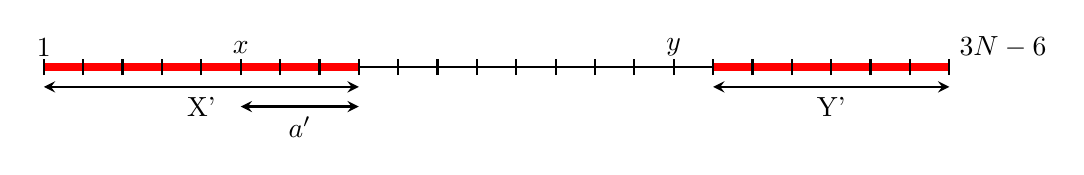
\begin{tikzpicture}[thick, scale=.5, >=stealth]
			\draw[black] (1, 0) -- (24, 0);
			\draw[line width=3pt, red] (1, 0) -- (9, 0) (18, 0) -- (24, 0);
			\foreach \x in {1, 2, ..., 24} {
				\draw (\x, -.2) -- (\x, .2);
			}
			\node at (6, .5) {$x$};
			\node at (17, .5) {$y$};
			\node at (1, .5) {$1$};
			\node[right] at (24, .5) {$3N-6$};
			\draw[<->] (6, -1) -- (9, -1) node[below, pos=.5] {$a'$};
			\draw[<->] (1, -.5) -- (9, -.5) node[below, pos=.5] {X'};
			\draw[<->] (18, -.5) -- (24, -.5) node[below, pos=.5] {Y'};
			\end{tikzpicture}
			
			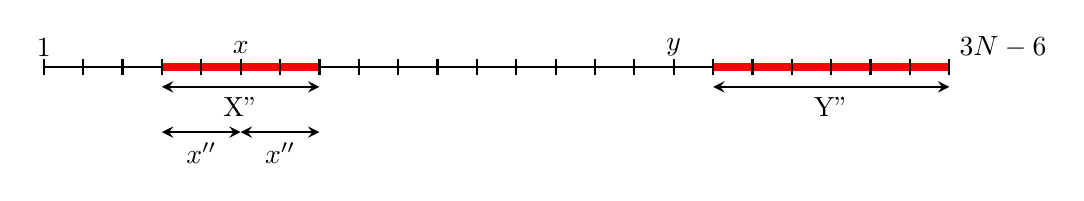
\begin{tikzpicture}[thick, scale=.5, >=stealth]
			\draw[black] (1, 0) -- (24, 0);
			\draw[line width=3pt, red] (4, 0) -- (8, 0) (18, 0) -- (24, 0);
			\foreach \x in {1, 2, ..., 24} {
				\draw (\x, -.2) -- (\x, .2);
			}
			\node at (6, .5) {$x$};
			\node at (17, .5) {$y$};
			\node at (1, .5) {$1$};
			\node[right] at (24, .5) {$3N-6$};
			\draw[<->] (4, -1.65) -- (6, -1.65) node[below, pos=.5] {$x''$};
			\draw[<->] (6, -1.65) -- (8, -1.65) node[below, pos=.5] {$x''$};
			\draw[<->] (18, -.5) -- (24, -.5) node[below, pos=.5] {Y''};
			\draw[<->] (4, -.5) -- (8, -.5) node[below, pos=.5] {X''};
			\end{tikzpicture}  
			
		\end{center}
		\caption{Selection of normal modes which are stored in the expression of the PES  : methodologies applied to realize the !truncation of the vibrational basis a) truncation n$^{\circ}$1 T’=X’+Y’; b) truncation n$^{\circ}$2 T’’=X’’+Y’’} \label{P1-fig2}
	\end{figure}
	
	\section{Results and Discussion}
	
	\subsection{Monomers}
	
	Benzothiophene (N=15) and dibenzothiophene (N=21) were chosen to test basis truncation. For each of these systems, a fully converged calculation of the variation-perturbation type was performed. The ensembles of the results obtained using the two truncated bases for the first twelve modes for benzothiophene are reported in Figures 3 (truncation n$^{\circ}$1) and 4 (truncation n$^{\circ}$2).  Of these twelve modes, modes 1, 2, 4, 5, 8, 10 and 12 occur in the C$_{s}$ plane whereas modes 3, 6, 7 and 9 are out of the C$_{s}$ plane. Since the outcomes of the test for the first nine modes of dibenzothiophene are comparable, they are provided in the supporting information as Figure S2.\\
	
	For truncation n$^{\circ}$1, the main results are reported here in Figures 3a - 3l. The information reported in these graphs represents the difference obtained on the calculation of a target vibration frequency in the reduced basis $\textbf{B’}$ from the result that would be obtained using the same variation–perturbation method with the full basis $\textbf{B}$. For example, the analysis of the target mode 1 (X’=1, Figure 3a) shows that the presence of only the higher-frequency $\omega_{CH}$ stretching modes suffices to describe the vibrational problem concerning this mode. This observation accords well with the hypothesis that only the large amplitude modes are strongly coupled with the elongation ones involving lighter atoms. The analysis of the other out-of-plane C$_{s}$ deformation modes (2, 4, 5 and 8) leads to similar conclusions. The results of the calculation on mode 2 are closer to those obtained for mode 1, which seems logical since these two vibrational modes are \textit{de facto} similar. Concerning modes 4 and 5, regardless of the number of selected states within the basis created from the X’ criterion, one can note the need to work with at least 13 modes on the Y’ basis in order to be as close as possible to the reference calculation. On the other hand, one observes that it is not necessary to take into account all the lower-frequency modes within the basis for the calculation to converge. This will be confirmed shortly by the analysis of the second truncation. Another striking observation also emerges from this analysis: if it is desirable to introduce some of the wagging, scissoring and stretching modes in the basis, the calculation will converge satisfactorily only if all of these modes are introduced at the beginning. Concerning mode 8, it can be noted that no truncation seems capable of leading to an acceptable convergence.\\
	
	We have added the results for modes 10 and 12 although they do not belong to the same low-frequency category considered in this study. These two modes lie at the interface between the low-frequency and the other modes. The main conclusion one can derive from them is that taking into account only the low frequency and $\omega_{CH}$ modes in the basis no longer suffices for convergence of the calculations. These conclusions are generalized beyond mode 12.\\
	
	The modes taking place in the plane of the molecule, \textit{i.e.} modes 3, 6, 7, 9 and 11, again corroborate our hypothesis; particularly for low-frequency mode 3. In addition, the $x’$ modes that are close to mode 3 seem to have no effect on the quality of the converged result. The descriptions of modes 6 and 7 show again that the results are not greatly dependent on the basis truncation unless all the $\omega_{CH}$ modes were previously selected. Analyzing the results for modes 9 and 11 leads to the same conclusion, except that a strong truncation of Y’ would cause a much more important deviation of the results from those observed for modes 3, 6 and 7.\\
	
	The analysis of the results concerning the second truncation allows one to confirm even more the observations just presented. Only the results obtained for the modes 4, 5, 6 and 8 are reported here. Representations of these results were added as a second layer to those obtained beforehand (Figure 4a-d insets); the two situations are connected by a series of points they share in common, \textit{i.e.} when $a’$=$x"$. The main information we can derive from these studies is that no low-frequency mode requires its closest neighbors to ensure a good convergence of the results. Every argument indicates that these modes are only coupled to those involving $\omega_{CH}$ stretching. Only modes 4 and 5 seem to slightly depend on each other.\\
	
	\begin{figure}[H]
		\begin{center}
			\begin{tabular}{c c c}
				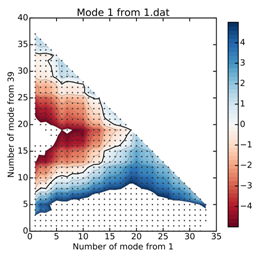
\includegraphics{image/P1-F311} & 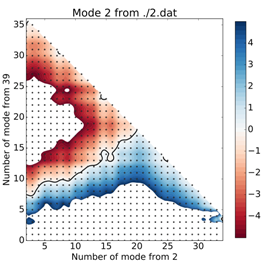
\includegraphics{image/P1-F312} &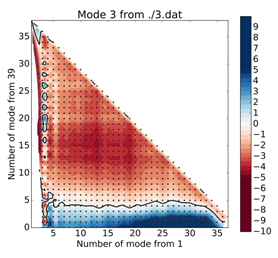
\includegraphics{image/P1-F313} \\
				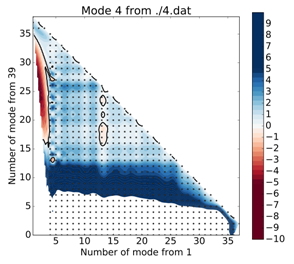
\includegraphics{image/P1-F321} & 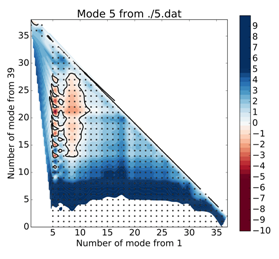
\includegraphics{image/P1-F322} & 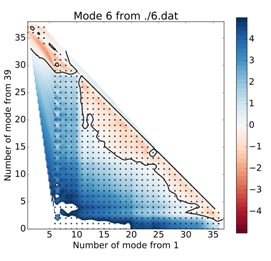
\includegraphics{image/P1-F323} \\
				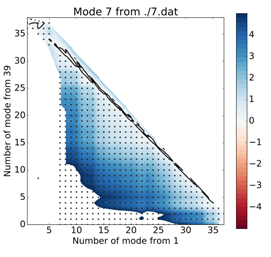
\includegraphics{image/P1-F331} & 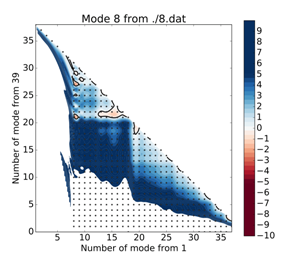
\includegraphics{image/P1-F332} & 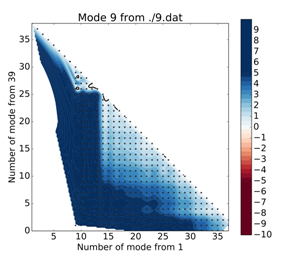
\includegraphics{image/P1-F333} \\
				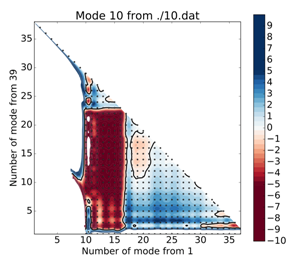
\includegraphics{image/P1-F341} & 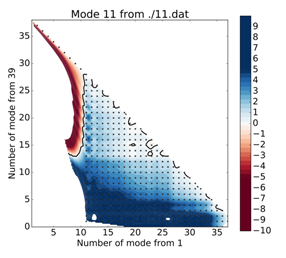
\includegraphics{image/P1-F342} & 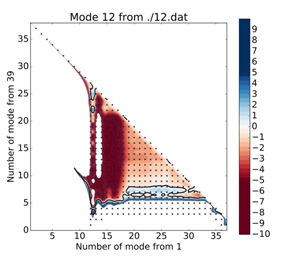
\includegraphics{image/P1-F343}\\   \label{P1-F3}
			\end{tabular}
		\end{center}
		\caption[Ensemble of results obtained using truncation n$^{\circ}$1 for the first twelve modes of a benzothiophene molecule]{Ensemble of results obtained using truncation n$^{\circ}$1 for the first twelve modes of a benzothiophene molecule. Mode 1: Figure 3a; Mode 2: Figure 3b … Mode 12: Figure 3l.
			In the $z$ axis are reported the values of the difference obtained on calculating a frequency without any truncation and the same frequency calculated in base $\textbf{B’}$ (T’=X’+Y’; X’ axis $x$; Y’ axis $y$; in accordance with the notation used in Figure \ref{P1-fig2}).}
	\end{figure}
	
	In summary, variational-perturbational studies using a truncated basis taking into account the closest neighbors of the low-frequency modes seems not to be an essential requirement for describing their vibrational properties as opposed to their coupling with the high-frequency stretching $\omega_{CH}$ modes. Finally, variational-pertubational studies using a truncated basis were performed for systems \textbf{1\textit{a}} (benzothiophene), \textbf{1\textit{b}} (dibenzothiophene), \textbf{1\textit{c}} (4,6-dimethyldibenzothiophene) and \textbf{1\textit{d}} (4-methyldibenzothiophene). The same was done for their dimers and compared against experimental results obtained by IR and Raman spectroscopy.
	
	
	\begin{figure}[H]
		\begin{center}
			\begin{tabular}{c c}
				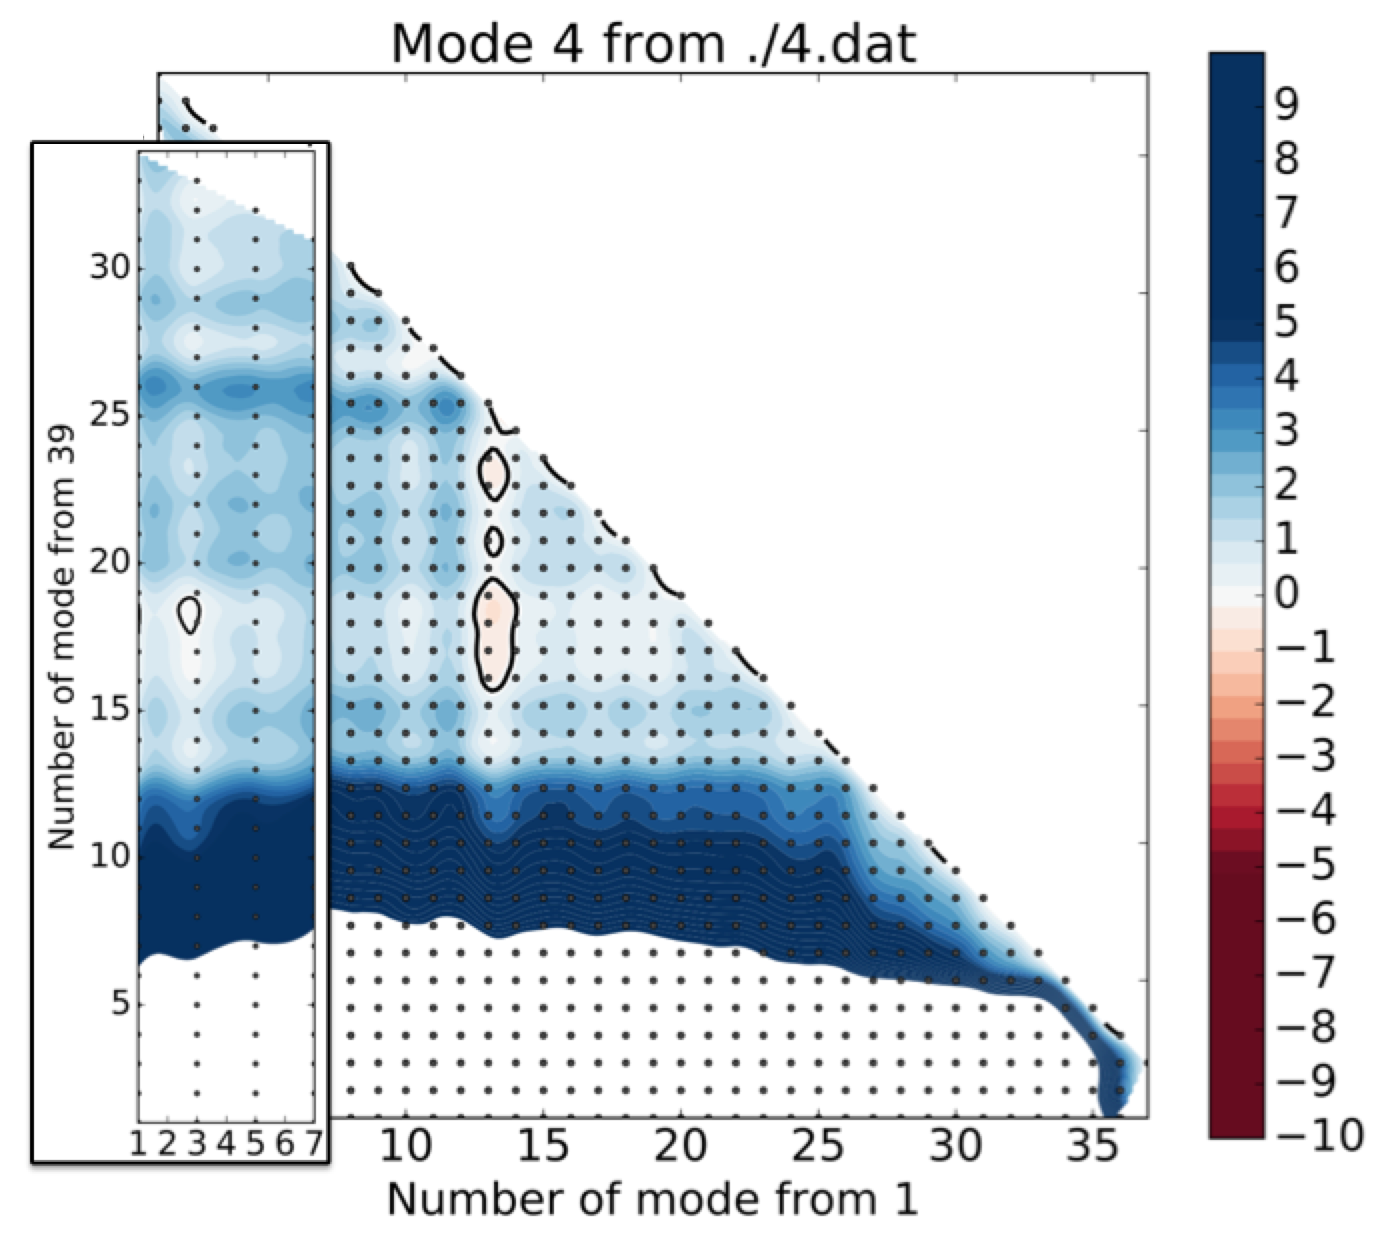
\includegraphics[scale=0.2]{image/P1-41} & 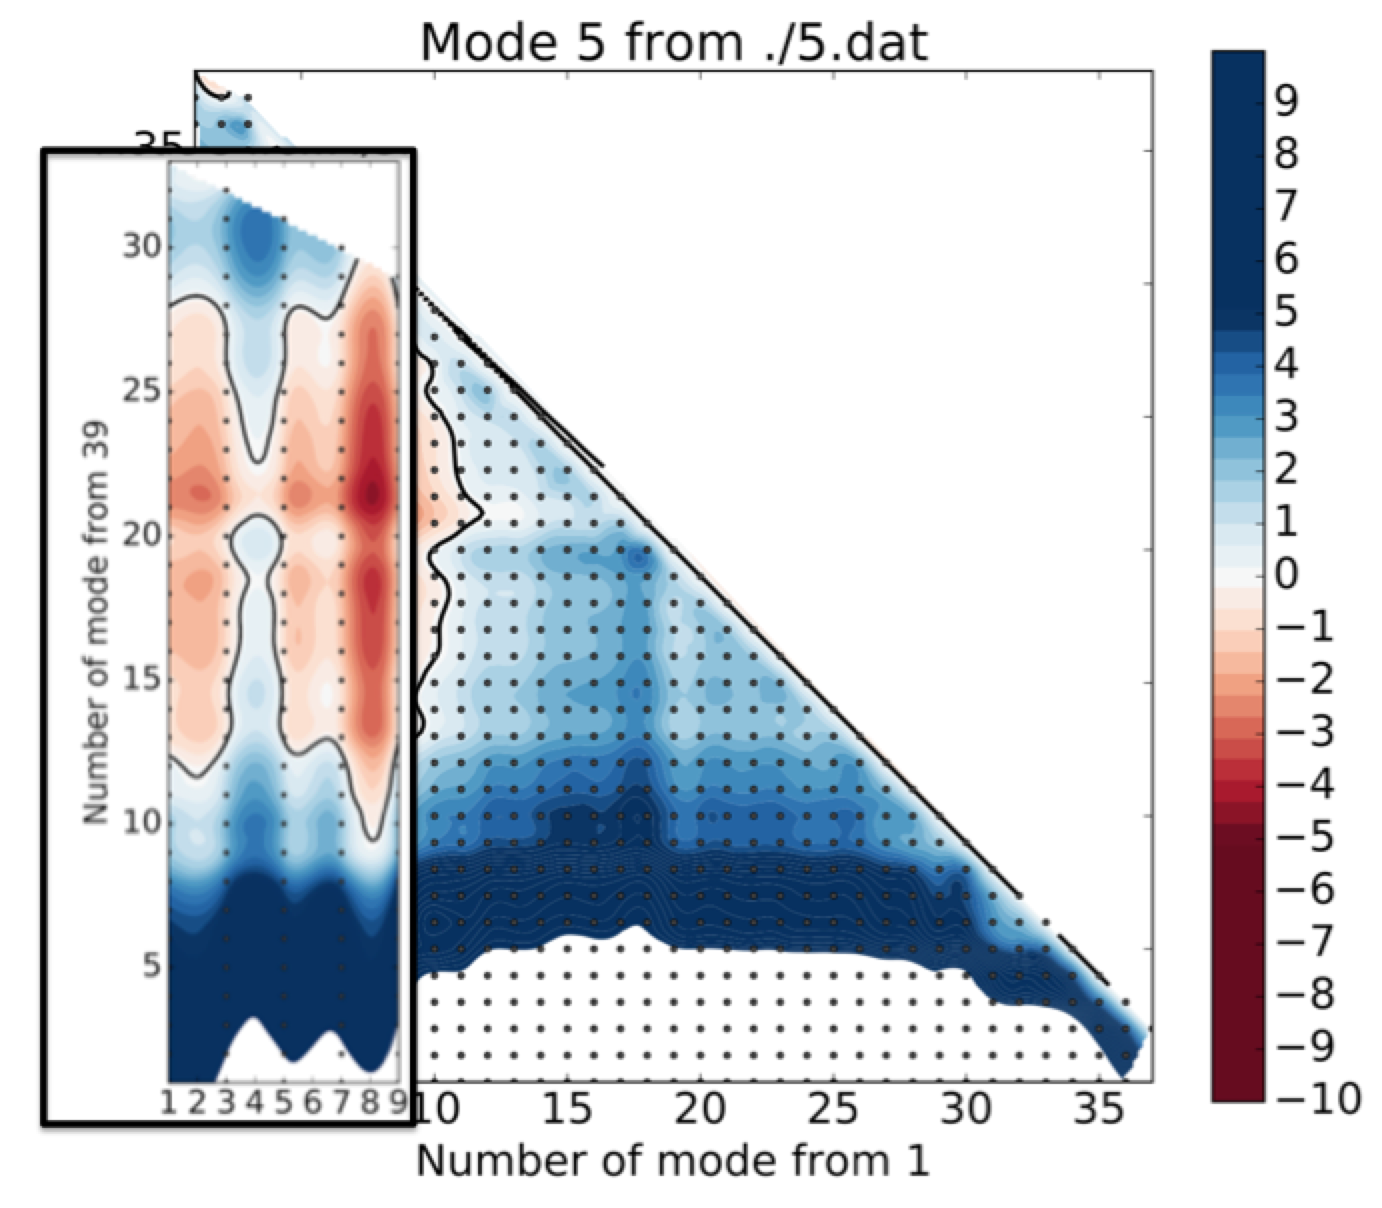
\includegraphics[scale=0.2]{image/P1-42}\\
				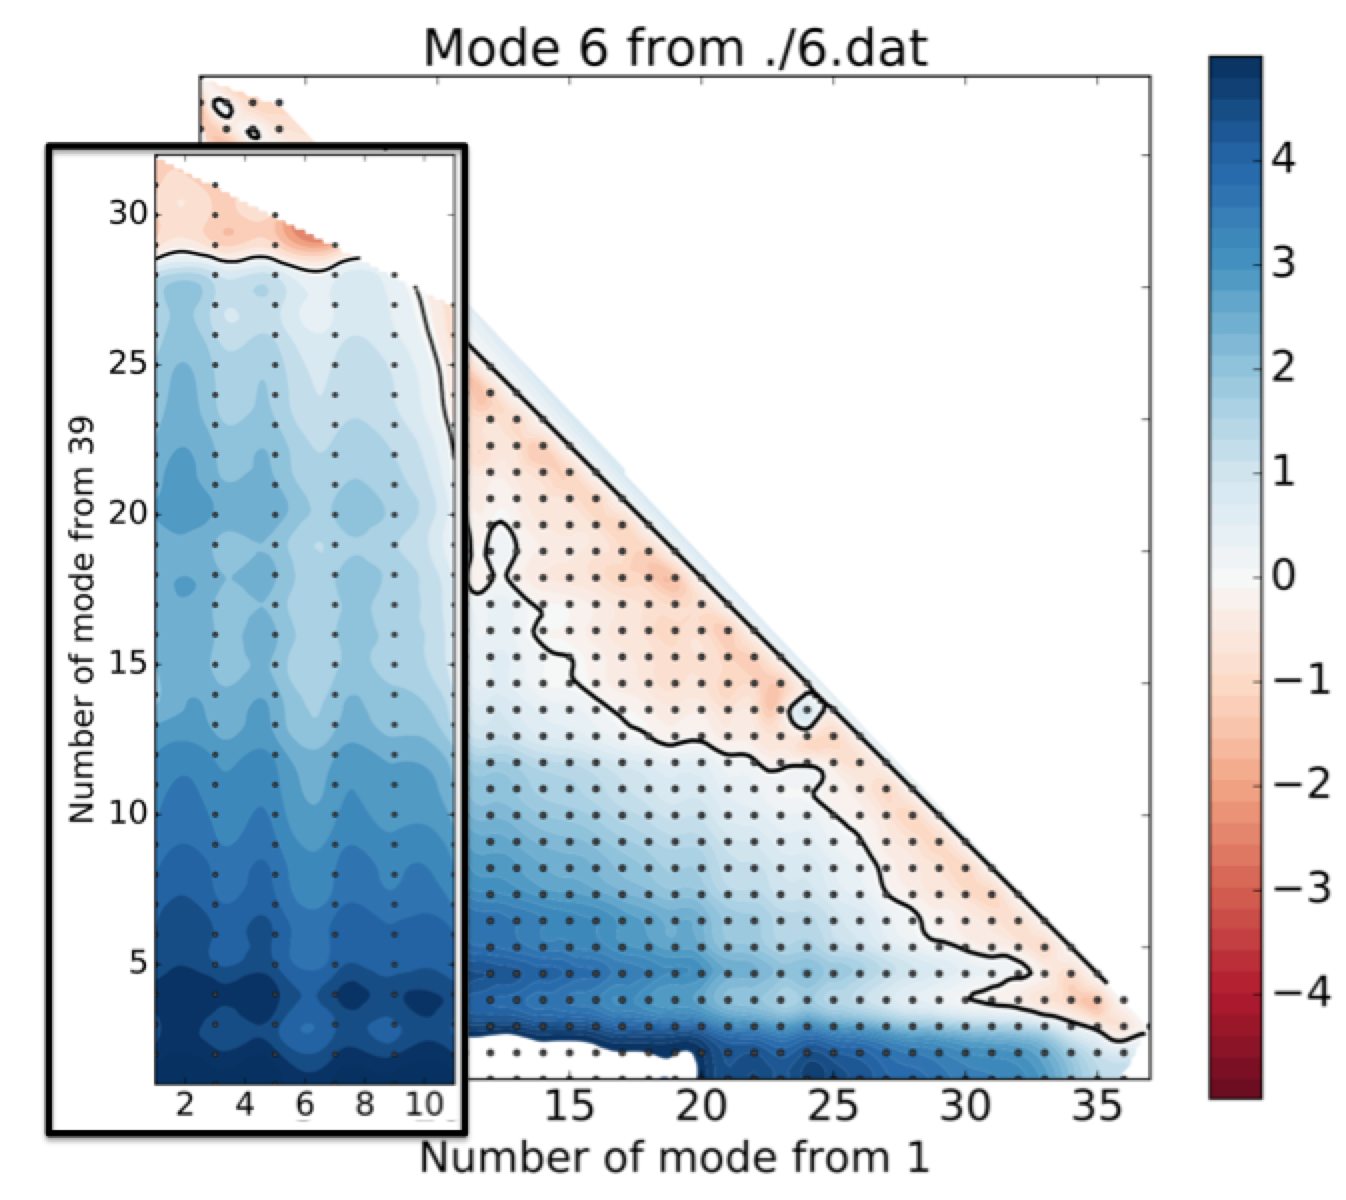
\includegraphics[scale=0.2]{image/P1-43} & 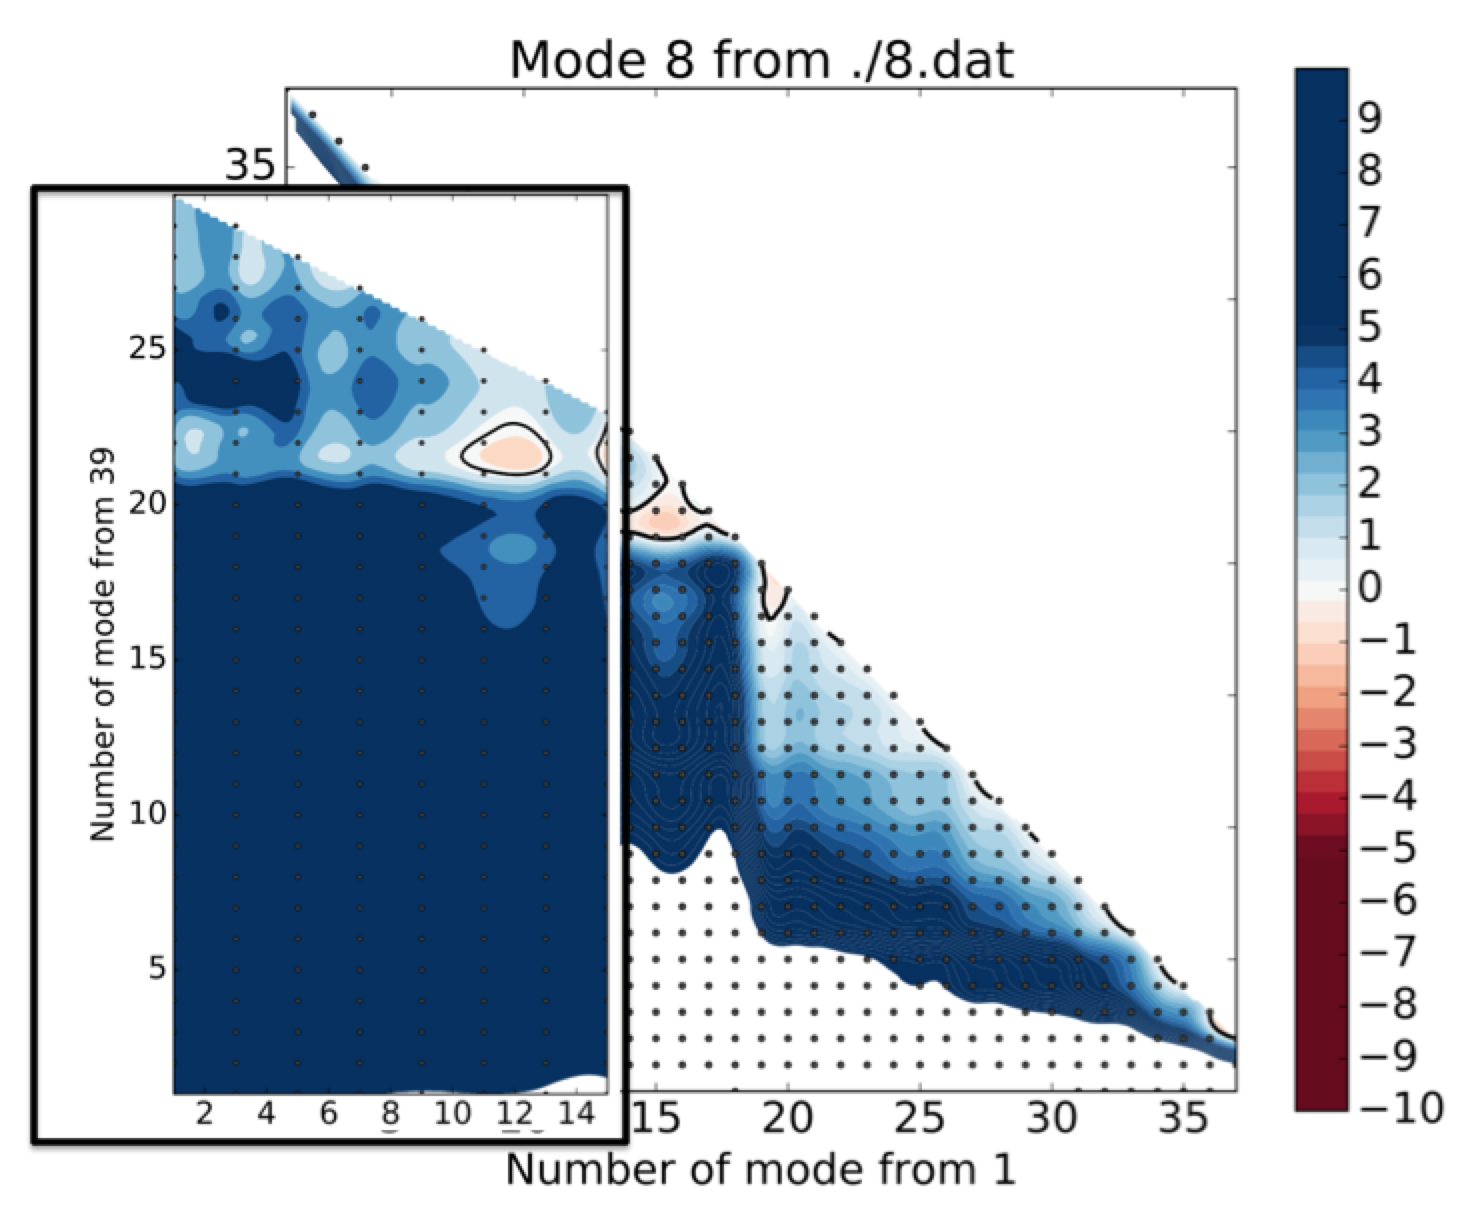
\includegraphics[scale=0.2]{image/P1-44}\\
			\end{tabular}
		\end{center}
		\caption[Ensemble of results using the truncation n$^{\circ}$2 for the first twelve vibration modes of a benzothiophene molecule]{Ensemble of results using the truncation n$^{\circ}$2 for the first twelve vibration modes of a benzothiophene molecule. Mode 4: Figure 4a; Mode 5: Figure 4b; Mode 6: Figure 4c;  Mode 8: Figure 4d.
			In the z axis are reported the values of the difference obtained on calculating a frequency without any truncation and the same frequency calculated in base $\textbf{B’’}$ (T’’=X’’+Y’’; X’’ axis $x$; Y’’=Y’ axis $y$; in accordance with the notation used in Figure \ref{P1-fig2}).}
	\end{figure}
	
	
	PA infrared and Raman spectra of \textbf{1\textit{b}} (dibenzothiophene), \textbf{1\textit{c}} (4,6-dimethyldibenzothiophene) and \textbf{1\textit{d}} (4-methyldibenzothiophene) were interpreted in light of the quantum chemistry calculations. Data for \textbf{1\textit{a}} (benzothiophene) were taken from the literature. The low-wavenumber and “fingerprint” regions (comprising, together, the 20–2000 cm$^{-1}$ range) were studied in detail in these investigations. In addition to the predicted infrared-active bands, the PA spectra of these hydrocarbons display many features due to overtones and combinations. Moreover, numerous Raman-active (gerade) vibrations also give rise to bands in the PA spectra, which thus convey considerable information regarding the structures of these compounds.\\
	
	
	\textit{Low wavenumber region (~100–700 cm$^{-1}$)}: both Raman and infrared spectroscopy results for \textbf{1\textit{a}} benzothiophene and \textbf{1\textit{b}} dibenzothiophene are reported in Tables 1 and 2. Raman and PA infrared results for \textbf{1\textit{c}} 4,6-dimethyldibenzothiophene and \textbf{1\textit{d}} 4-methyldibenzothiophene are given in Tables S8 and S9.\\
	
	
	For the benzothiophene molecule, the reported Raman spectrum has no significant features in this region. The IR spectrum is dominated by three intense bands at 471, 560 and 690 cm$^{-1}$ which are characteristic of wagging modes. Two other combination modes are IR-active. They are not easily detected since they have very low intensity and also due to the fact that the $\nu_{2}+ \nu_{5}$ mode has a signature very close to that of the active fundamental mode $\nu_{9}$. The analysis of the active modes of the dibenzothiophene molecule (Figure 5) shows that two of the three most intense wagging modes (\textit{obs} 497 and 704 cm$^{-1}$), which are, incidentally, characteristic of benzothiophene, can be clearly distinguished and do not allow one to easily separate the molecules from each other. However, one should note that a characteristic shift towards higher frequencies is found for these two modes of the dibenzothiophene system. Also note, in comparison to benzothiophene, an extinction (near 560 cm$^{-1}$) of the wagging signature because of symmetry induction and a new intense characteristic vibration located around 615 cm$^{-1}$. Moreover, the IR spectrum of this molecule for the region between 100 and 450 cm$^{-1}$ is more complex and richer in spectral features. As a matter of fact, other stronger and medium intensity modes signify the presence of the second benzyl moiety within the dibenzothiophene molecule. This observation agrees very well with our calculations. The analysis of the eigenfunctions generated by the variational-perturbational process shows that these modes are mainly developed on the basis of vibrational states that are characteristic of torsion ($\nu_{3}$(a$_{1}$) 213 cm$^{-1}$; \textit{calc} 217 cm$^{-1}$), breathing ($\nu_{4}$(b$_{1}$) 228 cm$^{-1}$; \textit{calc} 221 cm$^{-1}$) and ($\nu_{6}$(a$_{1}$) 404 cm$^{-1}$; \textit{calc} 416 cm$^{-1}$) and wagging ($\nu_{8}$(b$_{1}$) 425 cm$^{-1}$; \textit{calc} 433 cm$^{-1}$) combination modes of the benzenic rings. \\
	
	The Raman signature of the dibenzothiophene molecule is also more complex than that of benzothiophène. In the present context, this fact introduces only limited information since most of the active Raman modes are already the most intense and characteristic of the IR spectrum. All the other active modes have very low intensities which are again in agreement with our calculations. It is worth noting the confirmation provided by the Raman results concerning the shoulder observed in the IR spectrum around 419 cm$^{-1}$. 
	Similarly to the benzothiophene molecule two combination modes are foreseen by the calculations that can be, mainly for the $\nu_{2}+\nu_{8}$ mode, reasonably assigned experimentally.\\
	
	In addition to some frequency shifts, the spectra of both 4-methyldibenzothiophene and 4,6-dimethyldibenzothiophene exhibit important changes in the intensities of the vibrations in the 100 - 500 cm$^{-1}$ region as compared with the spectrum of dibenzothiophene. The clearest change occurs in the 400-460 cm$^{-1}$ region; the presence of substituents induces a significant change in intensity, ranging from very intense modes down to nearly zero (notably for the $\nu_{10}$ mode of 4-methyldibenzothiophene). These differences are even more pronounced in the Raman spectra. Whilst the presence of a single methyl group does not significantly change the Raman signature of the dibenzothiophene molecule, a second substitution in the 4,6 position does so very pronouncedly. The main change concerns the most characteristic mode of the di-substitution found at 598 cm$^{-1}$, which represents an in-phase breathing mode of the three rings.
	
	\begin{table}[H]
		\begin{center}
			\caption[Low wavenumber Raman and infrared spectra of benzothiophene]{Low wavenumber Raman and infrared spectra of benzothiophene (\textit{C$_s$ symmetry})}
			\begin{threeparttable}[b]
				\begin{tabular}{c c c c c}
					\toprule
					\multicolumn{2}{p{5cm}}{\centering \textbf{Observed$^{b}$}} & \multicolumn{3}{p{10cm}}{\centering \textbf{Calculation}} \\
					Raman & Infrared & Mode & $\omega^{a,c}$ & $\nu^{d}$ \\
					\midrule
					&  &   &    &   \\
					192 vw & 192 vw & $\nu_{1}$ (A") & 196 (0.22) [0.27] & 194 (0.20)\\
					& 198-212 w & $\nu_{2}$ (A") & 204 (4.11) [0.12] & 199 (2.97) \\
					340 vw & 340 vw & $\nu_{3}$ (A') & 351 (2.82) [2.11] & 345 (2.08) \\
					387 vw &   & $\nu_{1} + \nu_{2}$ &  & 391 (0.03) \\
					& 405-411 vw & $\nu_{4}$ (A") & 427 (3.45) [0.77] & 414 (2.50)\\
					& 471 m & $\nu_{5}$ (A") & 482 (5.88) [0.53] & 478 (6.02) \\
					491 vw & 491-497 vw & $\nu_{6}$ (A') & 500 (0.30) [10.64] & 494 (0.29) \\
					526 vw &  & $\nu_{7}$ (A') & 538 (0.25) [6.54] & 533 (0.36) \\
					& 558-564 m & $\nu_{8}$ (A") & 578 (5.88) [0.70] & 563 (5.24)\\
					& 669 vw & $\nu_{9}$ (A') & 683 (2.32) [1.47] & 675 (1.70)\\
					&  & $\nu_{2} + \nu_{5}$ &  & 679 (0.10) \\
					& 690 s & $\nu_{10}$ (A") & 710 (34.70) [0.23] & 692 (28.22)\\
					\bottomrule 
				\end{tabular}
				
				\begin{tablenotes}
					\item[a] Infrared intensities (in parentheses) in km/mol and Raman intensities [in brackets] in A$^{4}$/AMU.
					\item[b] Experimental data. Relative intensities: vw = very weak, w = weak, m = medium, s = strong, vs = very strong, sh = shoulder.
					\item[c] Unscaled DFT frequencies calculated using $\omega$B97X-D/6-311++G**.
					\item[d] Anharmonic $\omega$B97X-D/6-311++G** calculation using the A-VCI algorithm\cite{garnier2016adaptive}.
				\end{tablenotes}
			\end{threeparttable}
		\end{center}
	\end{table}
	
	
	\begin{figure}[H]
		\centering
		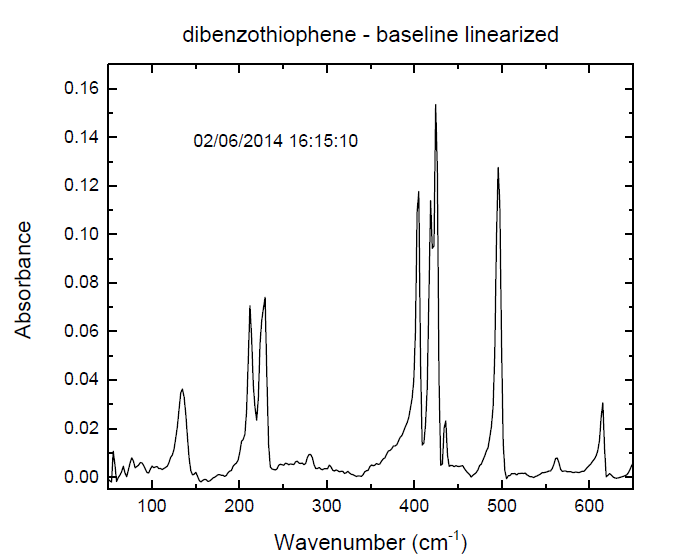
\includegraphics[scale=0.53]{image/Spectra-diben}  \label{P1-spectradiben}
		\caption{Far-infrared PA spectra of dibenzothiophene}
	\end{figure}
	
	
	
	\begin{table}[H]
		\begin{center}
			\caption[Low wavenumber Raman and infrared spectra of dibenzothiophene]{Low wavenumber Raman and infrared spectra of dibenzothiophene (\textit{C$_{2v}$ symmetry})}
			\begin{threeparttable}[b]
				\begin{tabular}{c c c c c}
					\toprule
					\multicolumn{2}{p{5cm}}{\centering \textbf{Observed$^{b}$}} & \multicolumn{3}{p{10cm}}{\centering \textbf{Calculation}} \\
					Raman & Infrared & Mode & $\omega^{a,c}$ & $\nu^{d}$ \\
					\midrule
					&  &   &    &   \\
					138 w & 135 m & $\nu_{1}$ (b$_{1}$) & 102 (1.54) [0.28] & 101 (0.66) \\
					171 w &  & $\nu_{2}$ (a$_{2}$) & 135 (0.00) [0.07] & 133 (0.01)\\
					217 m & 213 m & $\nu_{3}$ (a$_{1}$) & 217 (0.85) [1.25] & 208 (1.23) \\
					232 w & 228 m & $\nu_{4}$ (b$_{1}$) & 221 (1.46) [1.03] & 223 (1.42) \\
					& 269 vw &  &  &  \\
					282 w & 282 vw & $\nu_{5}$ (a$_{2}$) & 279 (0.00) [2.90] & 274 (0.00)\\
					287 sh & &  &  & \\
					410 s & 404 s & $\nu_{6}$ (a$_{1}$) & 416 (2.83) [13.05] & 409 (2.80)\\
					& 419 sh & $\nu_{7}$ (b$_{2}$) & 428 (0.14) [2.72] & 425 (0.15) \\
					419 m & 425 s & $\nu_{8}$ (b$_{1}$) & 433 (7.15) [0.01] & 425 (5.06) \\
					437 vw & 436 w & $\nu_{9}$ (a$_{2}$) & 444 (0.00) [0.06] & 438 (0.00) \\
					& 460 vw  &  &   & \\
					496 w & 497 s & $\nu_{10}$ ($_{1}$) & 505 (0.28) [4.76] & 499 (0.22) \\
					&  & $\nu_{12}$ (b$_{2}$) & 511 (1.23) [4.67] & 497 (1.48)\\
					504 vw & 512 w & $\nu_{11}$ (b$_{1}$) & 510 (2.74) [0.03] & 504 (1.18) \\
					& 565 w & $\nu_{2} + \nu_{8}$ (b$_{2}$) &   & 562 (0.12)\\
					&   &   $\nu_{13}$ (a$_{2}$) & 580 (0.00) [0.24] & 568 (0.00) \\
					& 615 m & $\nu_{14}$ (b$_{2}$) & 635 (5.09) [0.04] & 627 (4.62)\\
					& 667 w & $\nu_{17}$ (b$_{1}$) & 730 (0.82) [0.00] & 666 (0.15)\\
					&   &  $\nu_{3} + \nu_{10}$ (b$_{2}$) &  & 675 (0.01)\\
					703 s &704 vs &  $\nu_{15}$ (b$_{2}$) & 724 (6.53) [5.58] & 713 (6.43) \\
					\bottomrule 
				\end{tabular}
				
				\begin{tablenotes}
					\item[a] Infrared intensities (in parentheses) in km/mol and Raman intensities [in brackets] in A$^{4}$/AMU .
					\item[b] Experimental data from this work and ref\cite{bree1971vibrations}. Relative intensities: vw = very weak, w = weak, m = medium, s = strong, vs = very strong, sh = shoulder.
					\item[c] Unscaled DFT frequencies calculated using $\omega$B97X-D/6-311++G**.
					\item[d] Anharmonic $\omega$B97X-D/6-311++G** calculation using the A-VCI algorithm\cite{garnier2016adaptive}.
				\end{tablenotes}
			\end{threeparttable}
		\end{center}
	\end{table}
	
	
	
	
	
	\section*{Dimers}
	
	Characterization of the spectral signatures of “isolated” thiophene molecules constitutes the first part of this study. The second aim of this work lays in the identification and characterization of the IR and Raman signatures of the vibration modes at very low wavenumbers which are characteristics of associated systems such as dimers. In order to foresee and identify the spectral signatures typical of these interactions, we have first identified all the stable forms of benzothiophene (and its derivatives) dimers, \textit{i.e.}, \textbf{2\textit{a}} d-benzothiophene, \textbf{2\textit{b}} d-dibenzothiophene, \textbf{2\textit{c}} d-4-methyldibenzothiophene and \textbf{2\textit{d}} d-4,6-dimethylbenzothiophene. Among all the possible dimer configurations, eight types of benzothiophene dimers have been calculated; these are represented in Figure 6. In all tables and figures, the letter \textit{d} means dimer. The geometrical parameters are summarized in SI.  Our interest lies in $\pi$-stacking interactions, hence we have considered the molecules placed such that $\pi-\pi$ stacking interactions are favored.
	
	Although $\pi-\pi$ stacking interactions have been proven to be predominant, electrostatic interactions also induce specific configurations \cite{liu2014adjusting}. In order to validate the calculation method used, additional calculations using SAPT-DFT have been performed and geometrical parameters as well as interaction energies calculated with the two methods are compared. The energies for the different configurations of the benzothiophene molecule are reported in Table 3. The energies for all the configuration for the three other systems (\textbf{2\textit{b}}-\textbf{2\textit{c}}), the graphical representations and optimized structures can be found in the SI.
	
	
	\begin{figure}[H]
		\centering
		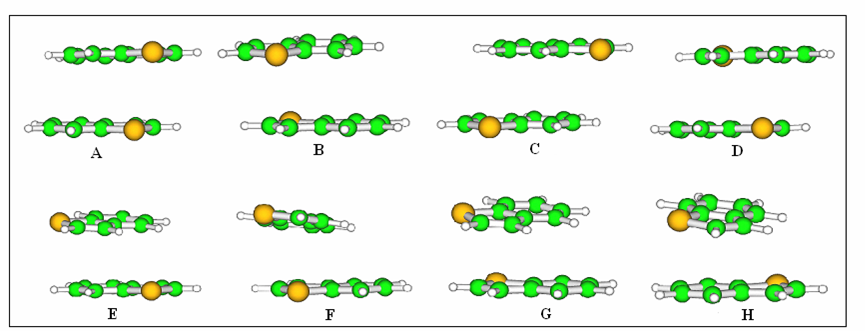
\includegraphics[scale=0.88]{image/P1-F6} \label{P1-F6}
		\caption{Configurations of benzothiophene dimers optimized at the $\omega$B97X-D/6-311++G** level of theory.}
	\end{figure}
	
	\begin{figure}[H]
		\centering
		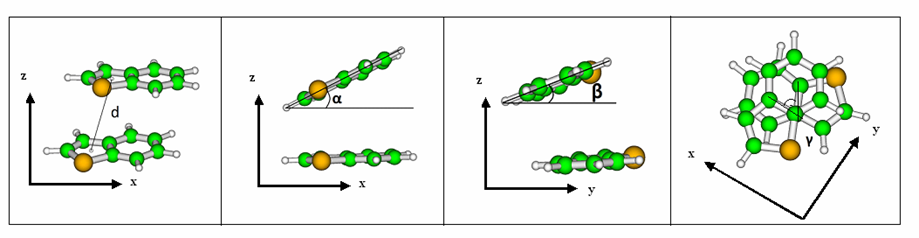
\includegraphics[scale=0.88]{image/P1-F7}  \label{P1-F7}
		\caption{Structural parameters of benzothiophene dimers}
	\end{figure}
	
	\noindent d = Intermolecular distance between thiophene rings center of benzothiophene dimers.\\
	$\alpha$ = Angle between the molecules inside $x$, $z$ plane. \\
	$\beta$ = Angle between the molecules inside $y$, $z$ plane.\\
	$\gamma$ = Angle of rotation in $z$ axis.\\
	
	
	\begin{table}[H]
		\caption[Interaction energies of benzothiophene dimers]{(a) Interaction energies of benzothiophene dimers (kcal/mol) in 8 different configurations using $\omega$B97X-D/6-311++G**, and compared with other methods. (b) Intermolecular distance between thiophene rings center of benzothiophene dimers (Å) (c) Angle between ring planes of benzothiophene dimers ($^{\circ}$) according to Figure 6. (d) Angle between ring planes of benzothiophene dimers ($^{\circ}$) according to Figure 6. Energies taking into account zero-point energy (ZPE) and Basis Set Superposition Error (BSSE) corrections.}
		\begin{center}
			\begin{threeparttable}[b]
				\resizebox{17cm}{!}{
					\begin{tabular}{c c c c c c c c c c}
						(a) &  &   &   &   &  &  &  &  & \\
						\toprule
						&	&  \textbf{A} & \textbf{B} & \textbf{C} & \textbf{D} & \textbf{E} & \textbf{F} & \textbf{G}& \textbf{H} \\
						\midrule
						\multicolumn{2}{p{5cm}}{\centering \small{$\omega$B97x-D/} \\ \small{6-311++G**}}  & -6.41 &  -7.05 & -6.83 & -7.11 & -7.23 & -7.01 & -7.02 & -7.00 \\
						\multicolumn{2}{p{5cm}}{\centering \small{DFT-SAPT(PBE0)} \\ \small{aug-cc pVTZ}}  & -5.33 & -5.73 & -5.56 & -5.95 & -5.83 & -5.87 & -5.72 & -5.63 \\
						\multicolumn{2}{p{5cm}}{\centering \small{B971/} \\ \small{6-31+G(d,p)-DCP$^{a}$}}  & -5.46 & -5.80 & -5.72 & -5.68 & -5.13 & -5.40 & -5.10 & -4.76 \\
						\bottomrule 
						\\
						\\
						\raggedleft (b)&  & & &   &  &  &  &   & \\
						\toprule
						& & \textbf{A} & \textbf{B} & \textbf{C} & \textbf{D} & \textbf{E} & \textbf{F} & \textbf{G}& \textbf{H} \\
						\midrule
						\multicolumn{2}{p{5cm}}{\centering \small{$\omega$B97x-D/} \\ \small{6-311++G**}}  & 3.94 & 3.81 & 5.28 & 3.72 & 4.49 & 3.56 & 3.74 & 4.37 \\
						\multicolumn{2}{p{5cm}}{\centering \small{DFT-SAPT(PBE0)} \\ \small{aug-cc pVTZ}}  & 3.98 & 3.80 & 5.16 & 3.75 & 4.53 & 3.65 & 3.70 & 4.30\\
						\multicolumn{2}{p{5cm}}{\centering \small{B971/} \\ \small{6-31+G(d,p)-DCP$^{a}$}} & 3.99 & 3.84 & 4.65 & 3.83 & 5.03 & 3.66 & 3.75 & 3.70\\
						\bottomrule
						\\
						\\
						(c) &   &   &   &  &  & &   &   & \\
						\toprule
						& &  \textbf{A} & \textbf{B} & \textbf{C} & \textbf{D} & \textbf{E} &  \textbf{F} & \textbf{G}& \textbf{H}  \\
						\midrule
						\multicolumn{1}{p{3cm}}{\centering \textbf{$\alpha$}} & &2.94 &1.73 &1.06 &0.44 &2.23  &4.38   &2.05  &6.37 \\
						\multicolumn{1}{p{3cm}}{\centering \textbf{$\beta$}}  & &3.59 &4.23 &3.14 &0.51 &5.07  &13.28  &9.03  &5.64 \\
						\multicolumn{1}{p{3cm}}{\centering \textbf{$\gamma$}} & &     &     &     &     &68.92 &100.06 &51.71 &77.25\\
						\bottomrule
						\\
						\\
						(d) &   &   &   &  &  & &   &   & \\
						\toprule
						& & \textbf{A} & \textbf{B} & \textbf{C} & \textbf{D} & \textbf{E}  &  \textbf{F} & \textbf{G}& \textbf{H} \\
						\midrule
						\multicolumn{1}{p{4cm}}{\centering \textbf{$\alpha$}} & &2.11 & 1.60 & 2.36 &1.49 & 3.50 & 2.66 & 11.90 & 7.97\\
						\multicolumn{1}{p{4cm}}{\centering \textbf{$\beta$}}& &4.00 & 3.67 &2.33 &2.00 &12.76 & 2.37 & 15.79 & 5.82\\
						\multicolumn{1}{p{4cm}}{\centering \textbf{$\gamma$}} & & &  &  &  &  108.52 & 105.27 & 107.62 & 51.44\\
						\bottomrule
					\end{tabular}}
					
					\begin{tablenotes}
						\item[a] ref\cite{mackie2010importance}
					\end{tablenotes}
				\end{threeparttable}
			\end{center}
			\label{P1-table3}
		\end{table}
		
		
		Eight conformations were highlighted for the benzothiophene dimer species. Benchmark energy calculations were performed using the DFT-SAPT(PBE0)/aug-cc pvtz level of theory. The $\omega$B97X-D/ 6-311++G** calculations, from which the vibrational calculations were performed taking into account both electrical and mechanical anharmonicities, lead to the same conclusions concerning the stability of these eight conformers (average deviation on the order of 1.25 kcal/mol). Regardless of the theory level that is employed, the two most stable conformations are \textbf{D} and \textbf{E}. In these conformations, the sulfur atoms are opposed to each other. This is also the case for the majority of the other systems studied in this work. The analysis of the energetic contributions linked to the intermolecular association phenomena is reported in Table 4.\\
		
		Before commenting on the results obtained by these contributions, one should recall the basis of the SAPT method used here. The van der Waals interactions, responsible for the cohesion of the dimers reported in this work, are clearly distinct to other types of long-range interactions. In the intermediate region that includes the minimum, it is very difficult to unequivocally decompose the total interaction energy into different contributions. Several decomposition schemes based on the Rayleigh-Schr\"{o}dinger perturbation theory have been proposed over the years. The principle of these approaches is the separation of the different contributions, such as electrostatic, induction and dispersion. On the other hand, the greatest drawback is the difficulty regarding convergence of the perturbative series (mainly the polarisation part, i.e., induction + dispersion), due to their truncation at low orders or their incompleteness. SAPT has been proposed to address this \cite{jeziorski1994perturbation}. In this approach, each of the aforementioned components should also include one exchange correction in order to take the antisymmetric nature of the wave function of the created complex into account. 
		
		A simple way to briefly present this theory is to start from a classical partition of a molecular dimer Hamiltonian of two monomers, say A and B:
		
		\begin{equation}
		H = H^{A} + H^{B} + V
		\end{equation}
		
		where $V$ stands for the intermolecular perturbation.\\
		
		The total Hamiltonian can be rewritten as:
		
		\begin{equation}
		H = H_{0}^{A} + W^{A} + H_{0}^{B} + W^{B} + V
		\end{equation}
		
		For which the $H_{0}^{A/B}$ terms are the Fock operators of both monomers A and B, $W^{A/B}$ stands for the monomer's intramolecular perturbation terms and can be understood as the « normal » correlation of each fragment (i.e. monomers A and B Moller-Plesset operators), and $V$ stands for the monomer's intermolecular perturbation term (i.e. the electrostatic attraction between A and B).\\
		
		The first perturbation level of order $N$ is obtained, in the first instance, from not considering the intramolecular correlation. The Rayleigh-Schr\"{o}dinger perturbation theory provides a series of well-known corrections for the interaction energy.\cite{chipman1973perturbation} However, it is usual to note that the perturbative series is seldom converged even though high-order terms (>2) are employed. Sometimes these series can even diverge. In order to avoid such behaviour, an asymptotic attenuation term is used for the energy in the form:
		
		\begin{equation}
		E_{int} = \sum_{n=1}^{N} E_{pol}^{(n)} + O(1/R^{2 (N+1)})
		\end{equation}
		
		Moreover, so that the anti-symmetric principle can be established within the SAPT approach, a classical anti-symmetrization operator is initially applied to the wave function of the systems allowing to establish the expression of the SRS (Symmetrized Rayleigh-Schr\"{o}dinger - which is the origin of the SAPT name) energy corrected from different perturbation orders up to a given $n$ large enough to contain all the long-range information.\\
		
		The second perturbation level of this methodology is obtained considering the intramolecular correlation (once the intermolecular perturbation has been treated accordingly). In this way, each intermolecular perturbation order $k$ one adds an intramolecular perturbative series respective to monomer A and B (of $m$ or $p$ order to develop the $W^{A}$ or $W^{B}$ operator, respectively). The summation over all the $m$ and $p$ orders leads to the following correction formula:
		
		\begin{equation}
		E_{pol}^{(k)} = \sum_{m,p} E_{pol}^{(kmp)}
		\end{equation}
		
		\begin{equation}
		E_{exch}^{(k)} = \sum_{m,p} E_{exch}^{(kmp)}
		\end{equation}
		
		which leads to a globally corrected interaction energy: 
		
		\begin{equation}
		E_{int} = \sum_{k=1}^{N} ( \sum_{m,p} E_{pol}^{(kmp)} + \sum_{m,p} E_{exch}^{(kmp)} ) + O(1/R^{2 (N+1)})
		\end{equation}
		
		or even:
		
		\begin{equation}
		E_{int} = E_{int} ({\scriptstyle HF,like}) + E_{corr-inter} + E_{corr-intra}
		\end{equation}
		
		with the term 
		
		\begin{equation}
		E_{int} ({\scriptstyle HF, like}) = E^{1,0,0}_{pol} + E^{1,0,0}_{exch} + E^{2,0,0}_{ind} + E^{2,0,0}_{exch-ind}
		\end{equation}
		
		representing the term calculated « without correlation » (from where the use of the ${\scriptstyle HF, like}$ acronym originates). 
		Moreover, one also has the corrected term to the intermolecular correlation :
		
		\begin{equation}
		E_{corr-inter} = E^{2,0,0}_{disp} + E^{2,0,0}_{exch-disp}
		\end{equation}
		
		One should note that the SAPT approach used for the study of non-polar complex systems (for which van der Waals forces are predominant) brings up little information and it is unnecessary to develop the perturbation beyond the second order.The so-obtained results (truncated at the order 2) for the four dimers $\textbf{B}$, $\textbf{D}$, $\textbf{E}$ and $\textbf{F}$ of the benzothiophene system are reported in Table 4. The very small numerical differences observed show that the nature of the interaction energies for different conformers does not make it possible to prove the existence of one as opposed to the others. Accordingly one could propose the concomitant presence of all these conformations as representative of inhomogeneous mixtures of asphaltenes, justifying the analysis made herein.
		
		\begin{spacing}{1.3}
			\begin{table}[H]
				\caption{Interaction energies components in kcal/mol of benzothiophene dimers using DFT-SAPT(PBE0)/aug-cc pVTZ}
				\begin{center}
					\begin{tabular}{c c c c c}
						\toprule
						&\textbf{B} &\textbf{D} &\textbf{E} &\textbf{F} \\
						\midrule
						\multicolumn{1}{p{5cm}}{\centering \textbf{$E^{1,0,0}_{pol}$}}       & -3.52     & -3.93     & -3.48     & -4.48     \\
						\multicolumn{1}{p{5cm}}{\centering \textbf{$E^{1,0,0}_{exch}$}}      & 10.99     & 11.04     & 10.76     & 10.41     \\
						\multicolumn{1}{p{5cm}}{\centering \textbf{$E^{2,0,0}_{ind}$}}       & -4.65     & -4.83     &-4.46      & -4.69     \\
						\multicolumn{1}{p{5cm}}{\centering \textbf{$E^{2,0,0}_{exch-ind}$}}  & 4.38      & 4.54      & 4.19      & 4.38      \\
						\multicolumn{1}{p{5cm}}{\centering \textbf{$E^{2,0,0}_{disp}$}}      & -14.01    & -13.78    & -13.97    & -12.37    \\
						\multicolumn{1}{p{5cm}}{\centering \textbf{$E^{2,0,0}_{exch-disp}$}} & 2.01      & 2.00      & 1.97      & 1.80      \\
						\multicolumn{1}{p{5cm}}{\centering \textbf{$E_{int} (\scriptstyle HF, like)$}}    & 7.20      & 6.82      & 7.01      & 5.62      \\
						\multicolumn{1}{p{5cm}}{\centering \textbf{$E_{corr-inter}$}}        & -12.00    & -11.78    & -12.00    & -10.57    \\
						\multicolumn{1}{p{5cm}}{\centering \textbf{$E_{corr-intra}$}}        & -0.93     & -0.99     & -0.84     & -0.92     \\
						\multicolumn{1}{p{5cm}}{\centering \textbf{$E_{int}$}}               & -5.73     & -5.95     & -5.83     & -5.87     \\
						\bottomrule
					\end{tabular}
				\end{center}
			\end{table}
		\end{spacing}
		
		In this work the Non-Covalent Interactions (NCI) formalism developed by Johnson and coworkers\cite{johnson2010revealing} was also used to analyze the energetic differences between all stable dimer forms. This formalism is based on the reduced electronic density gradient ($s$), a fundamental quantity in DFT theory which describes the deviation of the electronic density of a system ($\rho$) from the homogeneous case. Plotting $s$ versus $\rho$ reveals the basics of intramolecular interactions: for small $\rho$ and large $s$, one can identify the exponential decay of the density far from the nuclei. For small $s$ and large $\rho$, the points correspond to the covalent bond between the atoms. Situations where $\rho$ and $s$ are small are diagnostic for non-covalent interactions. To distinguish between attractive and repulsive non-covalent interactions, one needs to consider the Laplacian of the density ($\nabla^{2} \rho$).\\
		
		The components of the decomposition along the three coordinates are the three eigenvalues $\lambda_{i}$ of $\rho$'s Hessian matrix in a way that $\nabla^{2} \rho = \lambda_{1} + \lambda_{2} + \lambda_{3}$ is true for $\lambda_{3} \geq \lambda_{2} \geq \lambda_1$. Around the nuclei, there is a maximum for $\rho$ and all $\lambda_i$ are negative. For the interatomic regions between bonded atoms, the situation $\lambda_{3} > 0$ and $\lambda_{1}$ and $\lambda_{2} < 0$ exists. In this formalism, for covalent interactions, the negative contributions are dominant and the Laplacian is then negative. On the other hand, for non-covalent interactions, the Laplacian in the interatomic region is positive, irrespective of the bonding or non-bonding character of the interaction. Bonding interactions are, in this way, identified by a negative value of $\lambda_{2}$ whereas a positive value indicates non-bonding contacts. In other words, the sign of this eigenvalue is used to distinguish bonded $\lambda_{2} < 0$ and non-bonded interactions $\lambda_{2} > 0$.  $\rho$ itself indicates the strength of the interaction, as can be seen from Figures 8a-h.\\
		
		
		\begin{figure}[H]
			\begin{center}
				\begin{tabular}{c c c}
					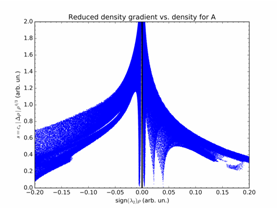
\includegraphics{image/P1-F811} & 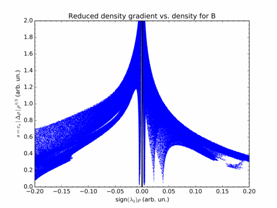
\includegraphics{image/P1-F812} & 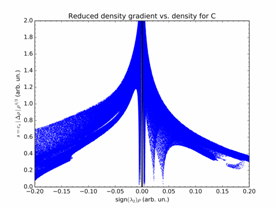
\includegraphics{image/P1-F813}\\
					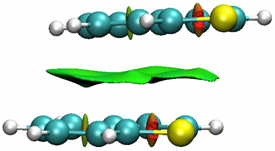
\includegraphics{image/P1-F821} & 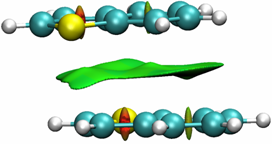
\includegraphics{image/P1-F822} & 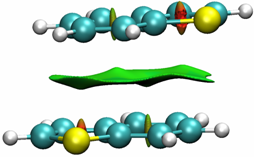
\includegraphics{image/P1-F823}\\
					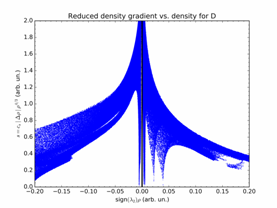
\includegraphics{image/P1-F831} & 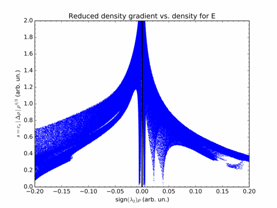
\includegraphics{image/P1-F832} & 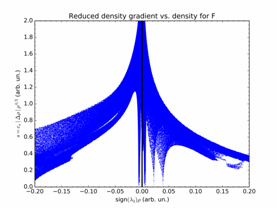
\includegraphics{image/P1-F833}\\
					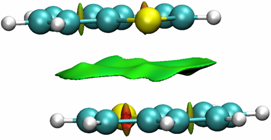
\includegraphics{image/P1-F841} & 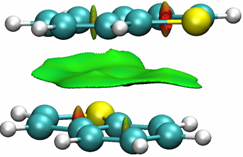
\includegraphics{image/P1-F842} & 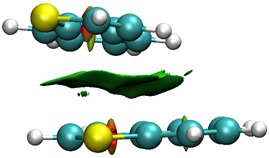
\includegraphics{image/P1-F843}\\
					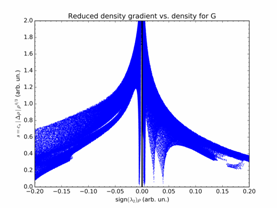
\includegraphics{image/P1-F851} & 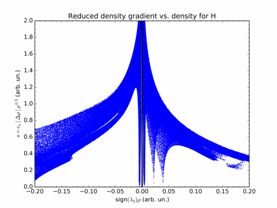
\includegraphics{image/P1-F852} & \\
					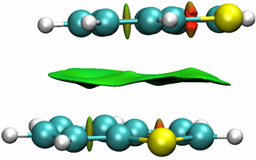
\includegraphics{image/P1-F861} & 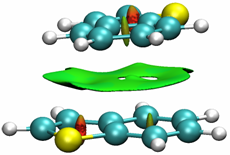
\includegraphics{image/P1-F862} & \\
				\end{tabular}
			\end{center}
			\caption{Plots of the electronic reduced gradient density's against against the density $\rho$ times the sign of $\lambda_{2}$}
		\end{figure}
		
		In this Figure, the low density, high gradient regions correspond to the exponential decay of the electronic density away from the nuclei of the molecules. The regions of gradient values around 0.5 arbitrary units and density values around $\pm$ 0.2 au correspond to the covalent interactions: in the positive region this is related to the repulsive character of the covalent intramolecular bonds and the negative region is correlated with attractive character.\\
		
		Moreover, the plots of these surfaces allow one to visualize the regions of space where the interactions are stronger. The color mapping indicates their repulsive character (towards red) or attractive (toward green). The intra-ring nuclear repulsion can be clearly distinguished from the interaction surfaces between the molecules of the dimer system in this way.\\
		
		From these plots, one can deduce that the conformations of the dimers have, to a limited extent, some influence on the non-covalent interactions. Although very little can be said from the reduced density gradient versus the density plots, the non-covalent surfaces show singular features for the studied conformers: conformer \textbf{F} has attractive interactions between the hydrogen atoms of one molecule and the carbon atoms of the other while conformer H has regions where no interaction takes place or where they mutually cancel (indicated by the holes on the surface). Moreover, analysis of the positioning of the intra-ring nuclear repulsion interactions shows that systems \textbf{C}, \textbf{D} and \textbf{E} have the surfaces of each benzyl or thiophene ring in opposition to each other. This increased interaction between the planes might indicate that the translational (sliding) vibration modes of one plane over the other should be slighty shifted to higher wavenumbers.\\
		
		\textit{Very Low wavenumber region (~30–100 cm$^{-1}$):}
		
		The first conclusion to be drawn from our calculations for all conformations for all species is that the very low wavenumber features in the spectra for all of the dimers are very similar to each other.\\
		
		
		This observation is also consistent with our spectra recorded between 5 and 26 cm$^{-1}$ for the dibenzothiophene \textbf{1\textit{b}},  4,6-dimethyldibenzothiophene \textbf{1\textit{c}} and 4-methyldibenzothiophene \textbf{1\textit{d}} systems (see Figure \ref{mole-verylow}). The assignation of the six libration modes of the most stable conformers for the four species (\textbf{2\textit{a}}-\textbf{2\textit{d}}) is reported in Table 5. The parameters of the variation-perturbation calculations used for each species are also reported in this table. These results show that the modes with the lowest wavenumbers, \textit{i.e.}, the sliding mode along the $xy$ plane (Figure 7) and the rotation around the main axis perpendicular to the plane of the isolated molecules (y direction) are mainly coupled; these modes are also coupled with several CH stretching modes. On the other hand, the other libration modes and, particularly, the sixth corresponding to the $\alpha$-type rocking mode are coupled, at the same time, to the stretching and wagging $\omega_{CH}$ modes. This justifies why these modes must imperatively be present in basis $\textbf{B’}$ (or $\textbf{B’’}$) in which the variation-perturbation work is performed so that convergence can be achieved. The calculated frequencies for each one of the dimers are reported in Table 6. Moreover, the results concerning the dibenzothiophene molecule are reported in Table 7 and compared to the only experimental data available in the literature and also to our PA measurements. All the results that were gathered from the literature do not lead to the same frequency due to the different methodologies in use but rather to a dispersion (around the frequency found by us). This is unsurprising since the measurement conditions differ among these experiments. The calculations performed for the dibenzothiophene dimer are in good agreement with the ensemble of experimental observations. They confirm that the very low-intensity bands observed experimentally are indeed the signatures of the intermolecular modes. The results in Table 6 also show that the rocking modes, found between 60 and 100 cm$^{-1}$, are not strongly dependent on the specie under study, and have more intense signatures than the libration modes. The rotation and sliding modes are much less intense and their locations are more dependent on the type of molecule. They are also more difficult to characterize in all types of spectroscopy: however, we have recently identified weak infrared absorption bands that may correspond to the sliding mode in spectra acquired using coherent synchrotron radiation (Figure \ref{mole-verylow}). Finally, the presence of one or several substituents at different positions on the molecule can also change the intensity of the signatures of the libration modes significantly, particularly for those implying, through vibration, the movement of the substituents towards each other, which gives rise to new intermolecular interactions.\\
		
		Previously, our group showed the extent to which these interactions play a significant role in the aggregation of molecules constituting the asphaltenes and the importance of characterizing them.\cite{silva2016molecular} Among these interactions, a non-negligible part consists in intermolecular interactions. Characterizing them through spectroscopy is then crucial for understanding the aggregation phenomena of asphaltene mixtures and, thus, estimating the energies required to separate them during the refining process and avoid the asphaltene sedimentation phenomenon widely observed in the pipelines. Our work using molecular dynamics sheds some light on the nature of the intermolecular interactions that can take place in the mixture for different heteroatoms, different lateral chains, etc. Among our future aims is the identification of characteristic features in vibrational spectra which permit identification of each interacting species for different heteroatoms and lateral chains that may be present in these aggregated systems.\\
		
		In summary, the present work shows that: 1) solving the vibrational Schr\"{o}dinger equation for isolated molecules allows one to identify, for molecules containing the sulfur heteroatom, the vibration modes for different molecular moieties as well as their singular spectroscopic properties; 2) utilizing both IR and Raman spectroscopy is very useful towards the full identification of these modes; 3) variation-pertubation calculations in the 100-700 cm$^{-1}$ region make it possible to complete the assignment of the modes of each monomer (which was previously initiated in the literature); 4) in the same region, vibrational modes of the dimers correspond to those of the isolated molecules making it possible to determine based solely on these modes, whether the molecules are interacting or not; 5) these intermolecular interaction modes are expected only at very low wavenumbers, and 6) in the region below 100 cm$^{-1}$, each molecule containing different configurations has characteristic signatures in the vibrational spectrum: these signatures arise from the sliding or rotation modes of one molecular plane with respect to another and can be in- or out-of-phase. Even though no general rule could be established concerning the behavior of these modes for different species or configurations, it is clear that their possible existence can serve as a marker for the presence or absence of intermolecular aggregation.\\ 
		
		Additionally use of the NCI formalism on a wide range of molecules cointaining different substituents and different heteroatoms should enable us to characterize the nature of these interactions in the future, and to quantify the energies involved in these interactions. This will make it possible to predict the behaviors for different molecular architectures and heteroatom arrangements.\\
		
		
		Finally, the description of the intermolecular modes chosen in this work is a first step of a project aimed at fully characterizing the aggregation interactions. In future work, we plan to a) perform solid state calculations, which are closer to actual experimental conditions since these interaction modes are linked to the deformations of the crystalline network of the solid (related results were already published by our group concerning the vibrational modes near 100 cm$^{-1}$ for a family of acenes); and b) study families of molecules with different chemical substituents and different heteroatoms (N, O and S).
		
		\begin{table}[H]
			\caption{Parameters used in the variation-perturbation process (values of X’ and Y as defined in Figure \ref{P1-fig2} parameters and dimension of of the variational  problem $\textbf{B’’}$) for each intermolecular mode of the four most stable dimers \textbf{2a-2d}}
			\begin{center}
				\resizebox{17.2cm}{!}{
					\begin{tabular}{c c c c c c c c c}
						\toprule
						& \multicolumn{2}{p{4cm}}{\centering \textbf{Benzothiophene}} & \multicolumn{2}{p{4cm}}{\centering \textbf{Dibenzothiophene}} & \multicolumn{2}{p{4cm}}{\centering \textbf{4-methyl} \\ \textbf{dibenzothiophene}} & \multicolumn{2}{p{4cm}}{\centering \textbf{4,6-dimethyl} \\ \textbf{dibenzothiophene}}\\
						Mode & type & X’’ ; Y’’ ; $\textbf{B’’}$ & type & X’’ ; Y’’ ; $\textbf{B’’}$ & type & X’’ ; Y’’ ; $\textbf{B’’}$ &type & X’’ ; Y’’ ; $\textbf{B’’}$\\ 
						\\
						1 & $x$,$y$  & 1 ; 7  ; 2500 & $\gamma$            &  1 ; 10 ;  3200 & $\gamma$            &  1 ; 14 ;  8100 & $\gamma$            &  1 ; 17 ; 10300 \\
						2 & $\gamma$ & 3 ; 7  ; 2500 & $x$,$y$             &  3 ; 10 ;  4100 & $x$,$y$             &  3 ; 14 ;  9000 & $x$,$y$             &  3 ; 17 ; 15100 \\
						3 & $x$,$y$  & 5 ; 7  ; 3000 & $x$,$y$             &  5 ; 10 ;  4500 & $x$,$y$             &  5 ; 14 ; 10500 & $x$,$y$             &  5 ; 17 ; 16600 \\
						4 & $\alpha$ & 7 ; 12 ; 3600 & $\alpha$            &  7 ; 15 ;  8800 & $\alpha$            &  7 ; 20 ; 12700 & $\alpha$            &  7 ; 23 ; 20500 \\
						5 & $\beta$  & 3 ; 12 ; 3500 & $\beta$             &  3 ; 15 ;  6300 & $\beta$             &  3 ; 20 ;  9900 & $\beta$             &  3 ; 23 ; 17400 \\
						6 & $\alpha$ & 9 ; 12 ; 4200 & $\alpha$ + $\omega$ & 11 ; 15 ; 15000 & $\alpha$ + $\omega$ & 11 ; 20 ; 17200 & $\alpha$ + $\omega$ & 11 ; 23 ; 24900 \\
						\bottomrule
					\end{tabular}}
				\end{center}
			\end{table}
			
			
			\begin{table}[H]
				\caption{calculated intermolecular vibrations modes of the four most stable dimers \textbf{2a-2d}}
				\begin{center}
					\resizebox{17.2cm}{!}{
						\begin{tabular}{c c c c c c c c c}
							\toprule
							& \multicolumn{2}{p{4cm}}{\centering \textbf{Benzothiophene}} & \multicolumn{2}{p{4cm}}{\centering \textbf{Dibenzothiophene}} & \multicolumn{2}{p{4cm}}{\centering \textbf{4-methyl} \\ \textbf{dibenzothiophene}} & \multicolumn{2}{p{4cm}}{\centering \textbf{4,6-dimethyl} \\ \textbf{dibenzothiophene}}\\
							Mode &  $\omega^{a}$ (I)$^{b}$ & $\nu^{a}$ & $\omega^{a}$ (I)$^{b}$ & $\nu^{a}$ & $\omega^{a}$ (I)$^{b}$ & $\nu^{a}$ & $\omega^{a}$ (I)$^{b}$ & $\nu^{a}$\\
							\\
							1 & 17 (0.02) &   &  18 (0.05) &  &  22 (0.01) &  &  17 (0.00)  &  \\
							2 & 18 (0.08) &  & 28 (0.01) & 24 & 36 (0.17) & 32 & 22 (0.01) & \\
							3 & 45 (0.06) & 39 & 36 (0.09) & 35 & 37 (0.01) & 31 & 41 (0.01) & 38\\
							4 & 67 (0.32) & 58 & 70 (0.32) & 66 & 65 (0.07) & 55 & 74 (0.52) & 66\\
							5 & 74 (0.02) & 67 & 89 (0.01) & 82 & 81 (0.03) & 67 & 83 (0.07) & 69\\
							6 & 91 (0.06) & 88 & 93 (0.56) & 92 & 96 (0.06) & 85 & 84 (0.01) & 78\\
							\bottomrule
						\end{tabular}}
						
						\begin{tablenotes}
							\item[a] : cm$^{-1}$
							\item[b] : km/mol
						\end{tablenotes}
					\end{center}
				\end{table}
				
				
				
				
				\begin{table}[H]
					\caption{Experimental and calculated intermolecular vibration modes (cm$^{-1}$) of dibenzothiophene dimer (\textbf{B}) }
					\begin{center}
						\begin{threeparttable}[b]
							\begin{tabular}{c c c c c c c c}
								\toprule
								& \multicolumn{2}{p{5cm}}{\centering \textbf{$\omega$B97x-D/6-311++G**}} & & & \textbf{IR$^{a}$} & \textbf{Raman$^{a}$} & \multicolumn{1}{p{2.5cm}}{\centering \textbf{IR$^{b}$} \\ \textbf{}}\\
								Mode & $\omega$ (I)$^{c}$ [I$^{Raman}$]$^{d}$ & $\nu$ & & & \multicolumn{3}{p{6cm}}{\centering $\nu$}\\
								\cline {1-3} \cline{6-8}
								\\
								1 & 18 (0.05) [0.62] &    & & &            &           &       \\
								2 & 28 (0.01) [7.96] & 24 & & &            &           &       \\
								3 & 36 (0.09) [9.15] & 35 & &  &53 w        & 48 - 49   & 56 w  \\
								4 & 70 (0.32) [0.51] & 66 & & &72 w        & 63        & 69 vw \\
								5 & 89 (0.01) [0.51] & 82 & & &89 vw       & 79 - 82   & 78 vw \\
								6 & 93 (0.56) [3.33] & 92 & & &104 - 101 w & 103 - 106 & 88 vw \\
								&                  &    & & &109 w       & 126       &       \\
								\bottomrule
							\end{tabular}
							
							\begin{tablenotes}
								\item[a] : liquid/crystal ref\cite{bree1971vibrations}.
								\item[b] : this work (crystal) 
								\item[c] : km/mol
								\item[d] : A$^{4}$/AMU
							\end{tablenotes}
						\end{threeparttable}
					\end{center}
				\end{table}
				
				\begin{figure}[H]
					\centering
					\subfigure[dibenzothiophene]{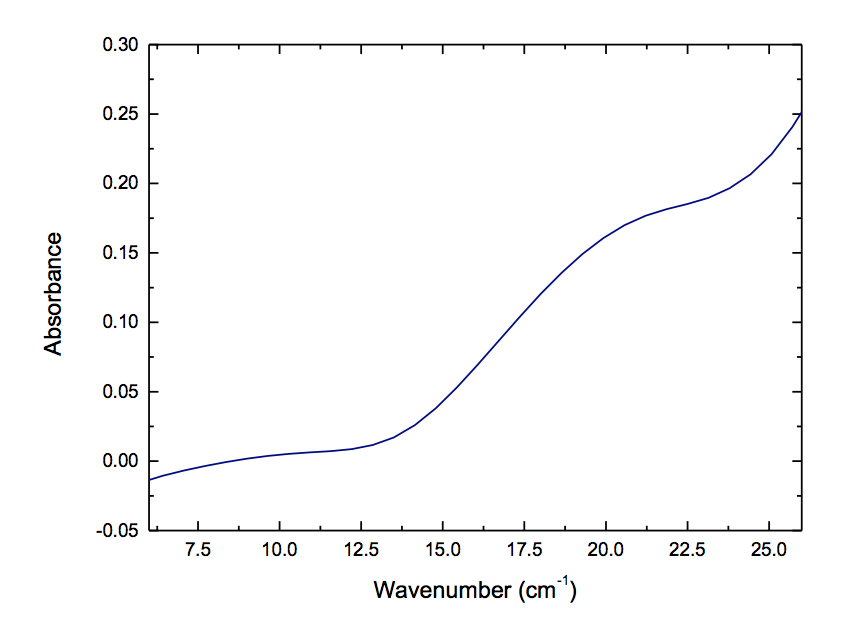
\includegraphics[scale=0.45]{image/dibenzo-verylow}}
					\subfigure[4,6-dimethyldibenzothiophene]{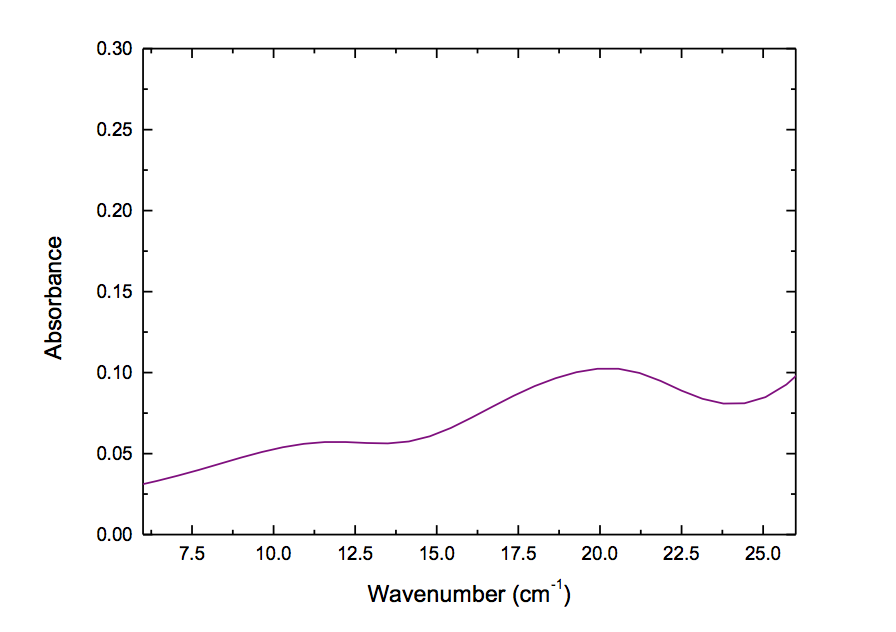
\includegraphics[scale=0.45]{image/4m-verylow}}
					\subfigure[4-methyldibenzothiophene]{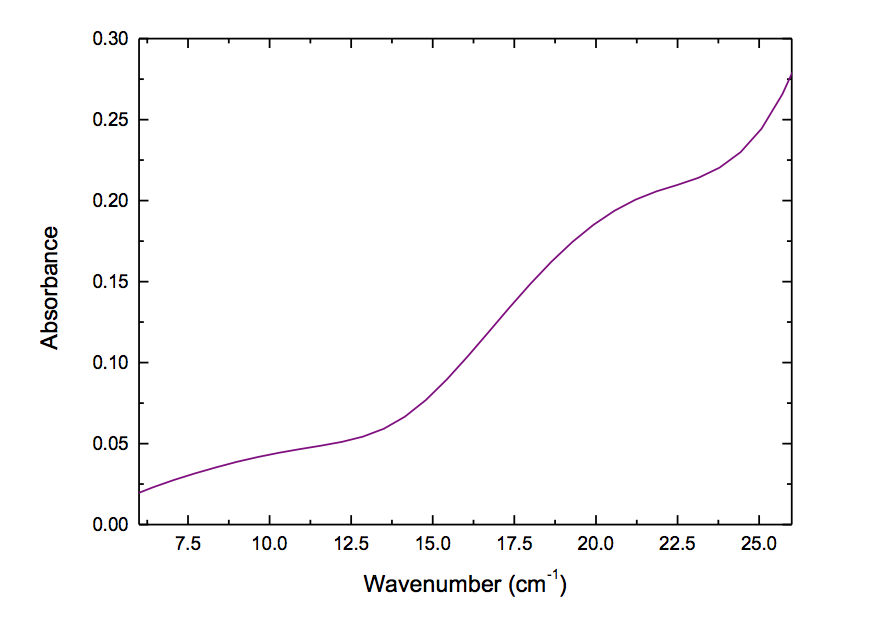
\includegraphics[scale=0.45]{image/46m-verylow}}
					\caption{Far-infrared spectra of dibenzothiophene \textbf{1\textit{b}}, 4,6-dimethyldibenzothiophene \textbf{1\textit{c}} and 4-methyldibenzothiophene \textbf{1\textit{d}}. Data were acquired using coherent synchrotron radiation and a Bruker IFS 125HR FT-IR spectrometer.}  \label{mole-verylow}
				\end{figure}
	
	